\documentclass{article}

% packages
  % basic stuff for rendering math
  \usepackage[letterpaper, top=1in, bottom=1in, left=1in, right=1in]{geometry}
  \usepackage[utf8]{inputenc}
  \usepackage[english]{babel}
  \usepackage{amsmath} 
  \usepackage{amssymb}
  % \usepackage{amsthm}

  % extra math symbols and utilities
  \usepackage{mathtools}        % for extra stuff like \coloneqq
  \usepackage{mathrsfs}         % for extra stuff like \mathsrc{}
  \usepackage{centernot}        % for the centernot arrow 
  \usepackage{bm}               % for better boldsymbol/mathbf 
  \usepackage{enumitem}         % better control over enumerate, itemize
  \usepackage{hyperref}         % for hypertext linking
  \usepackage{fancyvrb}          % for better verbatim environments
  \usepackage{newverbs}         % for texttt{}
  \usepackage{xcolor}           % for colored text 
  \usepackage{listings}         % to include code
  \usepackage{lstautogobble}    % helper package for code
  \usepackage{parcolumns}       % for side by side columns for two column code
  

  % page layout
  \usepackage{fancyhdr}         % for headers and footers 
  \usepackage{lastpage}         % to include last page number in footer 
  \usepackage{parskip}          % for no indentation and space between paragraphs    
  \usepackage[T1]{fontenc}      % to include \textbackslash
  \usepackage{footnote}
  \usepackage{etoolbox}

  % for custom environments
  \usepackage{tcolorbox}        % for better colored boxes in custom environments
  \tcbuselibrary{breakable}     % to allow tcolorboxes to break across pages

  % figures
  \usepackage{pgfplots}
  \pgfplotsset{compat=1.18}
  \usepackage{float}            % for [H] figure placement
  \usepackage{tikz}
  \usepackage{tikz-cd}
  \usepackage{circuitikz}
  \usetikzlibrary{arrows}
  \usetikzlibrary{positioning}
  \usetikzlibrary{calc}
  \usepackage{graphicx}
  \usepackage{caption} 
  \usepackage{subcaption}
  \captionsetup{font=small}

  % for tabular stuff 
  \usepackage{dcolumn}

  \usepackage[nottoc]{tocbibind}
  \pdfsuppresswarningpagegroup=1
  \hfuzz=5.002pt                % ignore overfull hbox badness warnings below this limit

% New and replaced operators
  \DeclareMathOperator{\Tr}{Tr}
  \DeclareMathOperator{\Sym}{Sym}
  \DeclareMathOperator{\Span}{span}
  \DeclareMathOperator{\std}{std}
  \DeclareMathOperator{\Cov}{Cov}
  \DeclareMathOperator{\Var}{Var}
  \DeclareMathOperator{\Corr}{Corr}
  \DeclareMathOperator{\pos}{pos}
  \DeclareMathOperator{\MV}{MV}
  \DeclareMathOperator{\V}{V}
  \DeclareMathOperator*{\argmin}{\arg\!\min}
  \DeclareMathOperator*{\argmax}{\arg\!\max}
  \newcommand{\ket}[1]{\ensuremath{\left|#1\right\rangle}}
  \newcommand{\bra}[1]{\ensuremath{\left\langle#1\right|}}
  \newcommand{\braket}[2]{\langle #1 | #2 \rangle}
  \newcommand{\qed}{\hfill$\blacksquare$}     % I like QED squares to be black

% Custom Environments
  \newtcolorbox[auto counter, number within=section]{question}[1][]
  {
    colframe = orange!25,
    colback  = orange!10,
    coltitle = orange!20!black,  
    breakable, 
    title = \textbf{Question \thetcbcounter ~(#1)}
  }

  \newtcolorbox[auto counter, number within=section]{exercise}[1][]
  {
    colframe = teal!25,
    colback  = teal!10,
    coltitle = teal!20!black,  
    breakable, 
    title = \textbf{Exercise \thetcbcounter ~(#1)}
  }
  \newtcolorbox[auto counter, number within=section]{solution}[1][]
  {
    colframe = violet!25,
    colback  = violet!10,
    coltitle = violet!20!black,  
    breakable, 
    title = \textbf{Solution \thetcbcounter}
  }
  \newtcolorbox[auto counter, number within=section]{lemma}[1][]
  {
    colframe = red!25,
    colback  = red!10,
    coltitle = red!20!black,  
    breakable, 
    title = \textbf{Lemma \thetcbcounter ~(#1)}
  }
  \newtcolorbox[auto counter, number within=section]{theorem}[1][]
  {
    colframe = red!25,
    colback  = red!10,
    coltitle = red!20!black,  
    breakable, 
    title = \textbf{Theorem \thetcbcounter ~(#1)}
  } 
  \newtcolorbox[auto counter, number within=section]{proposition}[1][]
  {
    colframe = red!25,
    colback  = red!10,
    coltitle = red!20!black,  
    breakable, 
    title = \textbf{Proposition \thetcbcounter ~(#1)}
  } 
  \newtcolorbox[auto counter, number within=section]{corollary}[1][]
  {
    colframe = red!25,
    colback  = red!10,
    coltitle = red!20!black,  
    breakable, 
    title = \textbf{Corollary \thetcbcounter ~(#1)}
  } 
  \newtcolorbox[auto counter, number within=section]{proof}[1][]
  {
    colframe = orange!25,
    colback  = orange!10,
    coltitle = orange!20!black,  
    breakable, 
    title = \textbf{Proof. }
  } 
  \newtcolorbox[auto counter, number within=section]{definition}[1][]
  {
    colframe = yellow!25,
    colback  = yellow!10,
    coltitle = yellow!20!black,  
    breakable, 
    title = \textbf{Definition \thetcbcounter ~(#1)}
  } 
  \newtcolorbox[auto counter, number within=section]{example}[1][]
  {
    colframe = blue!25,
    colback  = blue!10,
    coltitle = blue!20!black,  
    breakable, 
    title = \textbf{Example \thetcbcounter ~(#1)}
  } 
  \newtcolorbox[auto counter, number within=section]{code}[1][]
  {
    colframe = green!25,
    colback  = green!10,
    coltitle = green!20!black,  
    breakable, 
    title = \textbf{Code \thetcbcounter ~(#1)}
  } 

  \BeforeBeginEnvironment{example}{\savenotes}
  \AfterEndEnvironment{example}{\spewnotes}
  \BeforeBeginEnvironment{lemma}{\savenotes}
  \AfterEndEnvironment{lemma}{\spewnotes}
  \BeforeBeginEnvironment{theorem}{\savenotes}
  \AfterEndEnvironment{theorem}{\spewnotes}
  \BeforeBeginEnvironment{corollary}{\savenotes}
  \AfterEndEnvironment{corollary}{\spewnotes}
  \BeforeBeginEnvironment{proposition}{\savenotes}
  \AfterEndEnvironment{proposition}{\spewnotes}
  \BeforeBeginEnvironment{definition}{\savenotes}
  \AfterEndEnvironment{definition}{\spewnotes}
  \BeforeBeginEnvironment{exercise}{\savenotes}
  \AfterEndEnvironment{exercise}{\spewnotes}
  \BeforeBeginEnvironment{proof}{\savenotes}
  \AfterEndEnvironment{proof}{\spewnotes}
  \BeforeBeginEnvironment{solution}{\savenotes}
  \AfterEndEnvironment{solution}{\spewnotes}
  \BeforeBeginEnvironment{question}{\savenotes}
  \AfterEndEnvironment{question}{\spewnotes}
  \BeforeBeginEnvironment{code}{\savenotes}
  \AfterEndEnvironment{code}{\spewnotes}

  \definecolor{dkgreen}{rgb}{0,0.6,0}
  \definecolor{gray}{rgb}{0.5,0.5,0.5}
  \definecolor{mauve}{rgb}{0.58,0,0.82}
  \definecolor{lightgray}{gray}{0.93}

  % default options for listings (for code)
  \lstset{
    autogobble,
    frame=ltbr,
    language=C,                           % the language of the code
    aboveskip=3mm,
    belowskip=3mm,
    showstringspaces=false,
    columns=fullflexible,
    keepspaces=true,
    basicstyle={\small\ttfamily},
    numbers=left,
    firstnumber=1,                        % start line number at 1
    numberstyle=\tiny\color{gray},
    keywordstyle=\color{blue},
    commentstyle=\color{dkgreen},
    stringstyle=\color{mauve},
    backgroundcolor=\color{lightgray}, 
    breaklines=true,                      % break lines
    breakatwhitespace=true,
    tabsize=3, 
    xleftmargin=2em, 
    framexleftmargin=1.5em, 
    stepnumber=1
  }

% Page style
  \pagestyle{fancy}
  \fancyhead[L]{Algorithmic Trading}
  \fancyhead[C]{Muchang Bahng}
  \fancyhead[R]{Spring 2023}
  \fancyfoot[C]{\thepage / \pageref{LastPage}}
  \renewcommand{\footrulewidth}{0.4pt}          % the footer line should be 0.4pt wide
  \renewcommand{\thispagestyle}[1]{}  % needed to include headers in title page

\begin{document}

\title{Algorithmic Trading}
\author{Muchang Bahng}
\date{Spring 2023}

\maketitle
\tableofcontents
\pagebreak

A course on equity and derivative markets and relevant trading strategies. Contains information presented in Duke Math 585: Algorithmic Trading. 

\section{Stock Markets}

\textbf{Stocks} are a type of security that represents a share in the ownership of a corporation. That is, owning a stock is equivalent to owning its relative position in the company and its profits, and possibly voting rights. But what exactly does it mean to "own" a company? To explain this, we can interpret a business to be some sort of entity with input and output cash flows.

\begin{enumerate}
    \item The majority of the cash flows flowing into the business is the revenue earned from the goods and services that the business provides. 
    \item The majority of the cash flows flowing out of the business are the costs, such as COGS, employment compensation and benefits, operations, lawsuits, taxes, interest on debts, etc.
\end{enumerate}

Ideally, the company will have a net profit, or a net positive cash flow, which means that the cash flows in is greater than the cash flows out. All this profit, i.e. this extra money, now goes to the owners of this business through \textbf{dividends} (or may be reinvested into the company). Note that it is not the case that the profits go to the CEO. The CEO is a glorified version of an employee, but still in the end an employee, with an income just like every other employee, albeit a very high one. 
\begin{center}
    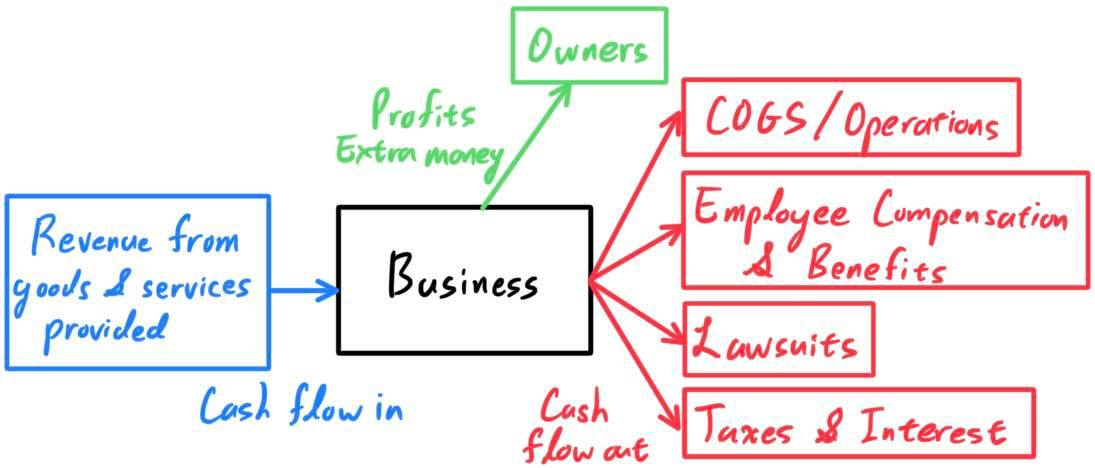
\includegraphics[scale=0.27]{img/Business_Cash_Flow.jpg}
\end{center}
Obviously, the owner has a bigger role to play rather than collect profits. They must also decide on things. But since there are usually many owners, these decisions are made through votes in meetings like the annual shareholder meeting. The ownership of a stock really possible rights to earn dividends and possible rights to vote. There is a much greater variety of stocks, but we will go through common ones.
\begin{enumerate}
    \item \textbf{Common stocks} are the most common type of stock. Common stock shareholders receive dividends in proportion to the amount of profit generated each year, and they have voting rights. They are usually the lowest priority over a company's income, after the creditors and preferred stock shareholders. 
    \item \textbf{Preferred stock} are much less common and liquid. Preferred stock shareholders receive fixed dividends and no voting rights. They receive payments after bondholders but before common shareholders. 
\end{enumerate}
Stocks may also have the following characteristics below. Generally, we work with common and preferred stocks, but other ones may be labeled using letters (e.g. Class A, Class B stocks) that have certain qualities mentioned below. 
\begin{enumerate}
    \item \textbf{Voting Power}: Nonvoting shares have no voting power while executive shares can be worth 10 votes. 
    \item \textbf{Payment Priority}: Deferred shares are set as a lower priority for dividends and corporate assets. 
    \item \textbf{Cumulative shares} can accumulate dividend payments that have been deferred due to low profits in the past. 
    \item \textbf{Convertible shares} can be converted into different forms of financial assets (e.g. preferred shares may be convertible into common ones, common shares may be convertible into corporate bonds).
\end{enumerate}
Note that if an entity (individual or organization) has the majority ownership or a \textbf{controlling interest} (at least 50\% in voting rights) of a company, then they have the power to do pretty much whatever they want with the company. 

\subsection{Primary Market: Private Funding, Public Offerings, Underwriting}

A company gets its funding from debt (e.g. bonds) and equity (stocks). If the prospect of paying interest on debts are not suitable, a company may issue stocks to investors. In other words, the company is selling parts of itself in exchange for capital. The number of shares, type of shares, and the prices for these shares is entirely determined by the seller and buyer. For example, a business may need to raise \$100 million in capital and can choose to issue 10 million shares at \$10 each.

For early-stage businesses, these are mainly funded by \textbf{venture capital} firms and \textbf{angel investors} (but is not limited to them) through different rounds roughly ordered: seed round, Series A, Series B, Series C, etc. After due diligence, these venture firms, as early investors, may get extra privileges, such as anti-dilution protection, guaranteed board seats, liquidation preferences, priority dividends. Note that upon multiple rounds of issuance, more and more stocks will circulate through more hands, causing \textbf{stock dilution}. No investor would want this and therefore stocks must be issued carefully. At this point, the ownership of a company is held within the hands of private individuals and firms.
\begin{center}
    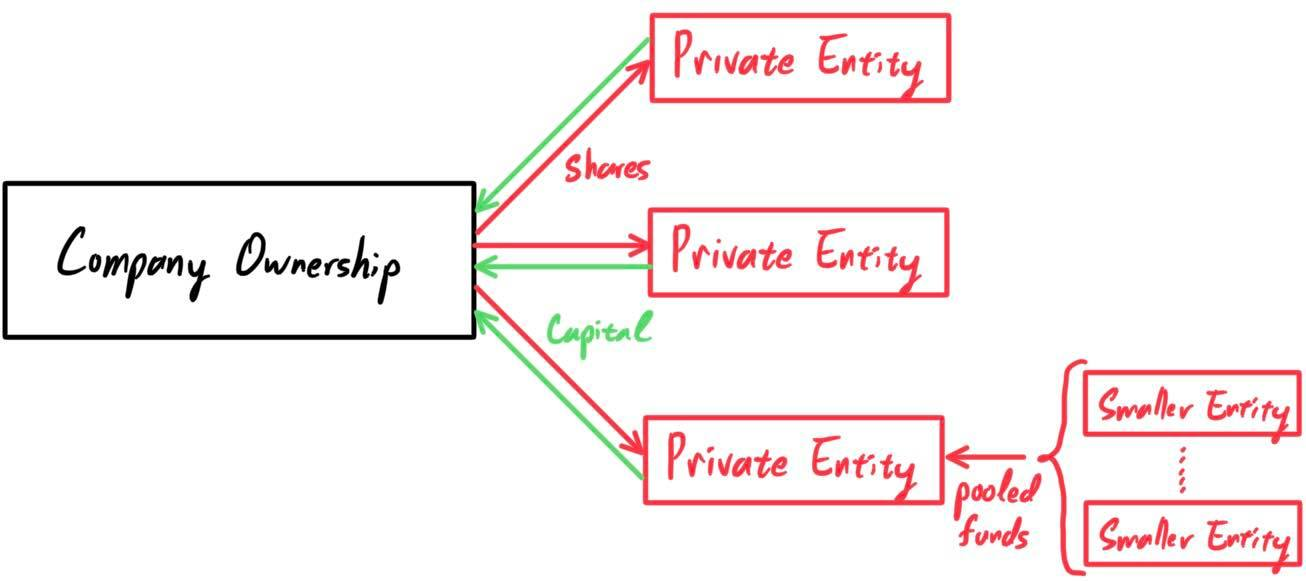
\includegraphics[scale=0.25]{img/company_in_private_hands.jpg}
\end{center}
One final characteristic to note is the \textbf{nominal value}, or \textbf{par value}, of a company's stock. Like the face value of a bond when issued, the nominal value of the stock is its stated value. It is an arbitrary value assigned for balance sheet purposes when the company is issuing share capital, and is typically \$1 or less. It has little to no bearing on the stock's market price, so no need to worry about this number.

Perhaps after a few years, the firm has grown to the point where funding on an even larger scale to support even more expansion is needed. Private sources may be too restrictive or small, and so companies may need to tap into the capital of the general public. Thus, they can do a \textbf{public offering}, an issuance of the stock to the general public rather than private entities. This process of an \textbf{initial public offering (IPO)} and the company being listed on a stock exchange is what is referred to as a company "going public." 
\begin{center}
    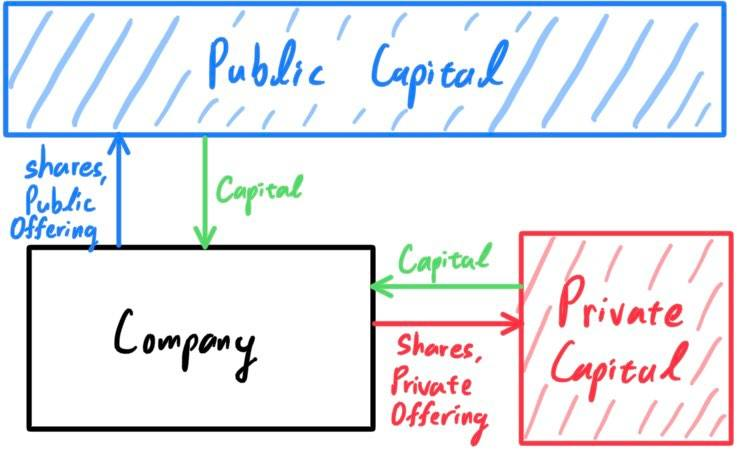
\includegraphics[scale=0.27]{img/Going_public.jpg}
\end{center}
Investment banks, through underwriting services, facilitate public offerings.
\begin{center}
    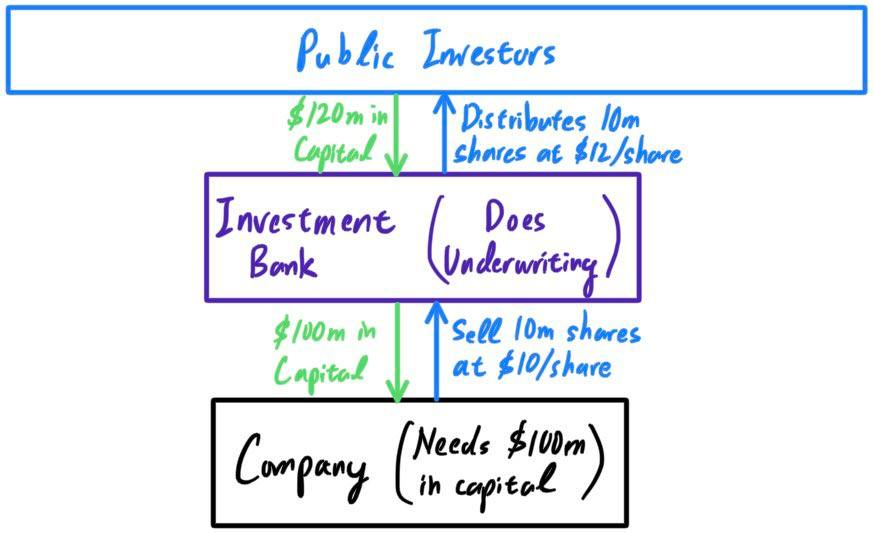
\includegraphics[scale=0.27]{img/Investment_bank_underwriting.jpg}
\end{center}

\subsubsection{Additional Actions on Stocks}
Throughout the years, companies may do the following: 
\begin{enumerate}
    \item Additional \textbf{stock issuance} to both public and private investors. 
    \item \textbf{Stock splits} to increase liquidity if the stock price is too high or for other reasons. \textbf{Reverse stock splits} may also be done.
    \item \textbf{Stock buyback} where the company uses its institutional funds to buy back shares from the market to increase its \textbf{treasury shares}. This may be used for anti-dilution purposes or to retain voting control. We can think of these as the opposite as a stock issuance, since treasury shares do not have dividend rights nor voting rights. 
    \item Issue \textbf{restricted stock units (RSUs)} to employees. The grant is restricted because it is subject to a vesting schedule, which can be based on length of employment or performance goals.
\end{enumerate}
With these, we can organize the number of stocks circulating in different levels, from biggest to smallest:
\begin{enumerate}
    \item Authorized shares refers to the maximum number of shares that a corporation is legally permitted to issue. Companies don't usually get close to this number due to market conditions, which will be explained later. 
    \item Shares issued refers to the total number of shares issued, including all public shares, private shares, and treasury shares. 
    \item Outstanding shares refer to a company's stock currently held by all shareholders, both public and private shares (including RSUs). It does not include treasury stocks however. 
    \item Floating shares are the shares considered available for the general public. Moreover, the floating percentage represents the portion of outstanding shares that are floating: 
    \[\text{Floating Percentage} = \frac{\text{Floating Shares}}{\text{Shares Outstanding}}\]
\end{enumerate}
\begin{center}
    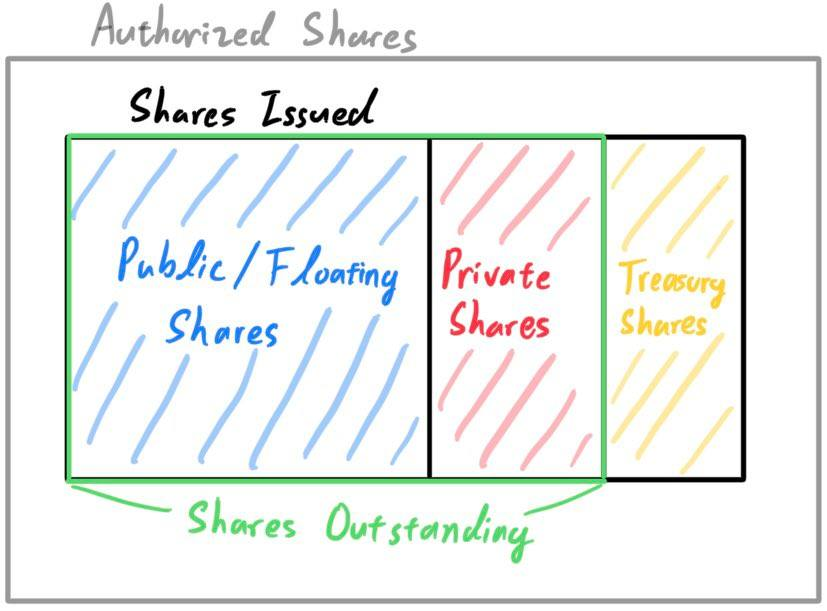
\includegraphics[scale=0.25]{img/Shares_Outstanding.jpg}
\end{center}

\subsection{Secondary Market}

\subsubsection{Involved Parties and Regulations}

Let us go through the basic construction of a market. When people want to buy and sell things, they must go to an \textbf{exchange}, which is literally a physical space that is leased to various parties (e.g. large banks, hedge funds) so that they can exchange goods. These exchanges also collect money through fees from companies to be listed on NYSE. There are two big exchanges, the NYSE and the NASDAQ, in the U.S., both located in New York. 

Us retail traders are not direct participants of the exchange; the parties that participate there are called the \textbf{market makers}, or \textbf{liquidity providers}. Market makers, usually large banks or financial institutions (like hedge funds), make sure that there is enough trading volume to ensure liquidity in the market. A buyer and a seller must meet together to complete a deal, and to ensure that this happens smoothly (i.e. provides liquidity), a market maker buys stocks (through the individual's brokerage) and sells them to the corresponding recipient. Essentially, they provide a pool of shares and act as intermediaries between them. They profit from the bid-ask spread, though sudden volatility is always a risk. For example, if a crash happens (i.e. a market maker buys a stock and it tanks before they can sell it), then the market makers get screwed because they are left with an undervalued stock. 

The trader cannot directly trade through the market makers. They must contact their \textbf{broker}, which is another company that acts as an intermediary. If I want to buy a stock, my buy order gets sent to my broker, which gets sent to the market makers, which pairs me up with a seller through their own broker, and the transaction is completed. These brokers make money through commissions from the traders and from trading in dark pools, which we'll talk about later. They also give access to traders the forecasts of analyst reports for companies and other research. 

\begin{center}
    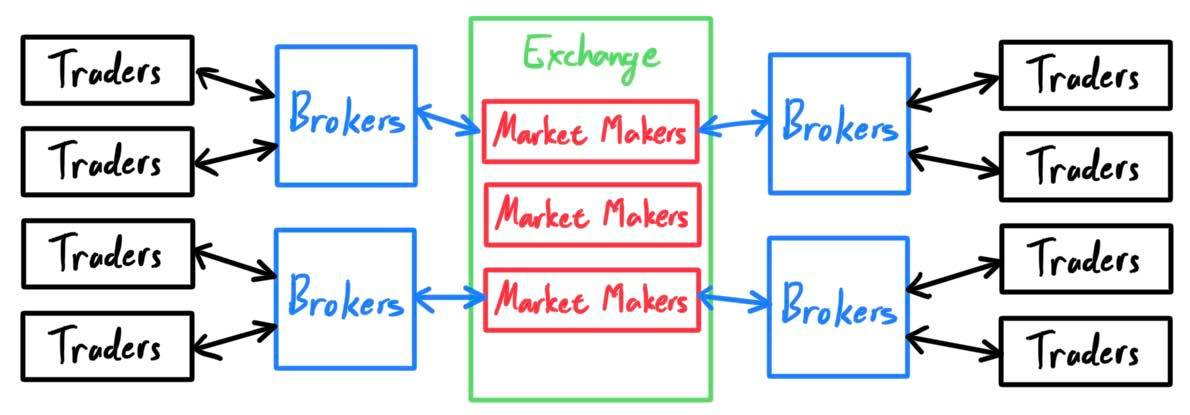
\includegraphics[scale=0.3]{img/exchange.jpg}
\end{center}

Clearly, there can be some shady stuff going on here, but luckily, the SEC and the FINRA consistently regulate the markets to ensure fairness for the little players (retail investors). One of the most important regulations is the 2005 Regulation NMS (National Market System), which required exchanges to publish the best bid and offer price for each stock, required them to route orders to the trading venue with the best price, and had set the minimal price quotation increment to \$0.01. This ensured transparency and protection of the investor with the best price execution (but this can be taken advantage of by high frequency traders). 


\subsubsection{Stock Orders}

The two most common orders one can do is the market order and the limit order. 
\begin{enumerate}
    \item A \textbf{market order} just buys or sells securities at the market price. This ensures that the transaction will be completed, but the price at which you buy or sell may not be what you want. 
    \item A \textbf{limit order} buys or sells at least at a certain price. It ensures that you get the price you want for a transaction, but it may not be carried out always. 
    \begin{enumerate}
        \item A buy limit order at \$X tells the broker to buy a stock at \$X or lower. 
        \item A sell limit order at \$x tells the broker to sell a stock at \$ or higher. 
    \end{enumerate}
    \item A \textbf{stop loss order} is used to limit an individual's loss or lock in a profit on a stock position. 
    \begin{enumerate}
        \item If an investor buys a stock at \$100, they can make a stop loss at \$95. This means that when the stock price reaches \$95, then it will automatically place a market order to sell the stock (the price may not be fulfilled at exactly \$95 due to volatility). 
        \item If an investor has a short position, on the stock, then they can put a stop loss order at \$105, essentially telling the broker to buy the stock when the price reaches \$105. 
    \end{enumerate}
\end{enumerate}

In addition to holding a long position, we can \textbf{short sell}, or short, a stock. Given that 100 shares of AAPL are each priced at \$100, we can borrow shares from some investor (probably an institutional investor), sell it on the market for \$100, and hope for the price to drop so we can buy it back. This is pretty symmetric to longing a stock, and many hedge funds use a \textbf{long-short equity strategy} involving a combination of longs and shorts, but there are additional risks. 
\begin{enumerate}
    \item You must pay additional interest for borrowing stocks. 
    \item Your potential losses is not bounded. 
    \item If you have too much unrealized losses as the stock price goes up, then you may not have enough \textbf{margin} (cash) in your account to even buy back to stock. To prevent this, your broker may issue a \textbf{margin call}, which forces you to buy the stocks back, locking in your loss, unless you add more capital to your account. This margin call may not happen right at the point when your free cash is not enough to buy back all shorted shares. Rather, your brokerage may run some complicated statistical simulations, calculate some confidence interval, and then decide on a threshold that determines whether you will get a margin call. 
\end{enumerate}
The third risk is the deadliest, and at worst, you can get \textbf{short-squeezed}. Let's explain how this works. Say you and a bunch of other investors shorted GME. GME prices start going up, and it reaches a point where some investors have to buy back the GME shares due to a margin call. The investors buy back the GME at market price, which adds more orders to the limit order book, causing the price to go even higher. This higher price causes more short-sellers to buy back GME due to additional margin calls, causing GME to go even higher, and so on. This positive feedback loop is extremely deadly, killing off many short sellers. 

Sometimes, the ethics of short selling are called into question. People who want to ban shorting state that short selling can drive down the stock price, which can be bad because it doesn’t spur the economy and reduces optimism in stock markets. Short selling means that stock is being borrowed and sold on the market, increasing supply, and therefore (all else being equal) decreasing price. However, these short sellers keep the stock price more in line with reality, and bad companies are punished by short sellers. 

Finally, the entities that drive this short selling are \textbf{prime brokers}, which are large financial institutions (usually investment banks) that provide financial management to mainly hedge funds. They act on behalf of the short seller, locating the assets to be sold short for them and providing them with a margin account (which must hold capital to the sum of at least 150\% of the value of the initial transaction). They enable hedge funds to borrow large amounts of stocks from institutional investors to short-sell them and allow them to access large amounts of margin from commercial banks. The prime brokerage makes money through commissions. Prime brokers can also loan capital to investors to increase their leverage, and they also provide financial research and analytics to their clients. 

\subsubsection{Stock Prices and Limit Order Books}

Now how is the share price determined? There are two large paradigms for this. The first is the \textbf{fundamental approach}, which attempts to calculate the intrinsic value fo the company by calculating its discounted future cash flows. 
\[\mathrm{Present Value} = \sum_{n=1}^\infty \frac{\text{Cash Flow}_1}{(1 + R)^n}\]
However, we will concern ourselves with the second approach: the \textbf{market approach}, which claims that the stock price is determined by supply and demand. This can be seen by looking at the \textbf{limit order book} (LoB), which shows all pending limit orders at the current time. This allows us to see where the prices are concentrated at and how strong the demand is versus the supply. In the diagram below, the right side represent the sell limit orders while the left side represents the buy limit orders. If we submit 50 buy market orders, then the best price is executed. 
\begin{center}
    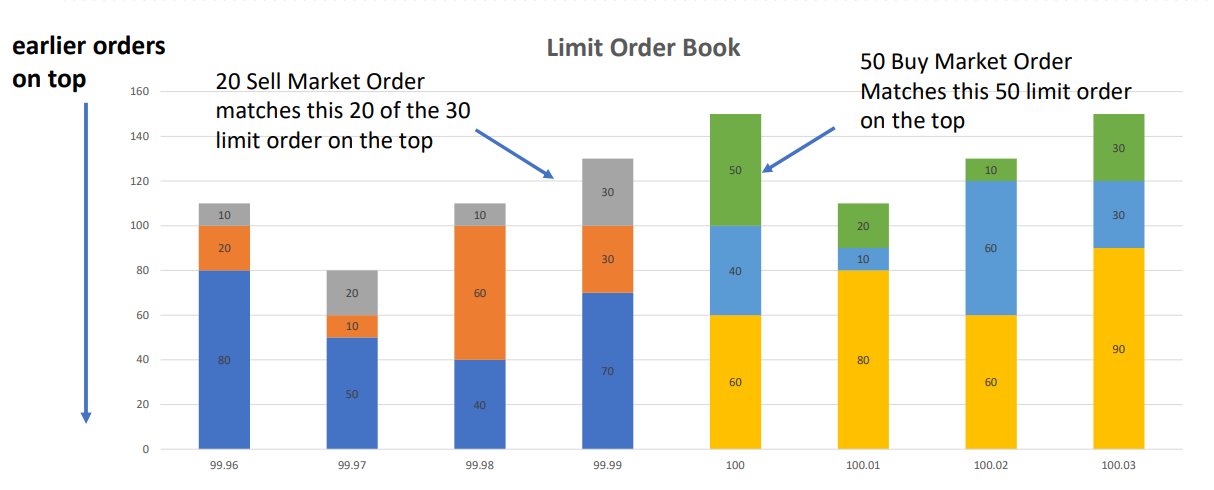
\includegraphics[scale=0.3]{img/limit_order_book.png}
\end{center}
The market makers profit off of the \textbf{bid-ask spread}, which is the difference in the buy and sell price. If a seller wants to sell at \$99.99 and a buyer wants to buy at \$100.00, then the market maker can buy the stock from the seller for \$99.99 and sell it to the buyer at \$100.00, making a \$0.01 profit. 

\subsubsection{High Frequency Trading}

A significant mover of markets are \textbf{high frequency traders}, or HFTs. HFT is a type of algorithmic trading that are characterized by high speeds and high turnover rates. It is the primary type of algorithmic trading and consists of about 50\% of all equity trades in the U.S. There is an average of about 1 trader per 10 milliseconds. Whether HFT is beneficial is very controversial: 
\begin{enumerate}
    \item Some argue that it is good since it increases liquidity and lowers transaction costs for retail investors. Even for potentially risky stocks (e.g. very overvalued), HFTs will always make a market out of them. 
    \item It can be considered unfair because it gives a huge advantage to HFT firms through front-running and other short-term strategies. This also increases the probability of \textbf{flash-crashes} (e.g. 2010 flash crash). 
\end{enumerate}
Unsurprisingly, many HFT firms are market makers due to their ability to provide liquidity. 

The primary form of HFT is \textbf{scalping}, which profits off of small price changes. The multiple benefits and drawbacks are easy to spot: 
\begin{enumerate}
    \item It requires a strict exit strategy since one large loss could eliminate the many small gains the trader worked to obtain. 
    \item It also requires a much higher ratio of winning trades vs losing ones, while keeping profits roughly equal or slightly bigger than losses. 
    \item A brief exposure to the market diminishes the probability of running into an adverse event like a crash. 
    \item Smaller moves are easier to obtain, so there are plenty of opportunities to exploit. 
\end{enumerate}
This strategy is extremely sensitive that even the physical location of the firm relative to the exchange matters. Heavy money in infrastructure is invested. 


\subsubsection{Market Manipulation}

\textbf{Market manipulation} is a type of market abuse where there is a deliberate attempt to interfere with the free and fair operation of the market. 
\begin{enumerate}
    \item \textbf{Stock Bashing}: Creating fake news about a company to drive prices down and get shares for a cheaper price. The perpetrators sometimes work directly for Investor Relations firms who have convertible notes that convert cor more shares the lower the bid or ask price is. Thus, the bashers can drive the stock price down by convincing shareholders that they have bought a worthless security. 
    \item \textbf{Pump and Dump}: Misleadingly promoting a company to drive share prices up (the "pump", e.g. with bogus emails to investors). When the stock price reaches a target level, the promoter sells their shares (the "dump"). 
    
    \item \textbf{Spoofing / Layering}: When a trader places a bid or offer on a stock with the intent to cancel before execution, these fake order trick other market participants by creating the false impression of heavy buying or selling pressure. Layering is an advanced form of spoofing with multiple orders that are "layered." For example, let's say that I want to buy stock XYZ, which is priced at \$100. If I wanted to use layering, I would put a sell order of 100 stocks at \$101, 100 at \$102, and 100 at \$103. An algorithm or trader might see this and believe that there is selling pressure and jump in front of these orders before they go down. They might sell at the market price of \$100, which may bring the price of XYZ a bit lower, to say \$99.95. I can buy at this price now. 
    
    \item \textbf{Front Running / Tailgating}: This is the practice of entering into a transaction that takes advantage of nonpublic knowledge of a large "block" pending transaction that will influence the price of an underlying security. Say a broker gets an order from a major client to buy 500,000 shares of XYZ Co. Such a huge purchase is bound to drive up the price of the stock immediately, at least in the short term. The broker sets aside the request for a minute and first buys some XYZ stock for their own personal portfolio or through accounts of relatives. Then the client's order is put through. The broker immediately sells the XYZ shares and pockets a profit. This can be used by HFT firms, since with the knowledge of large block buy orders from institutions, they can "buy up" all the orders in the market and sell it at a slightly higher price to the institutions. 
    
    \item \textbf{Quote Stuffing}: This is the practice of quickly entering and withdrawing a large number of orders in an attempt to flood the market, used by HFT firms. This can create confusion in the market (by filling up bandwidth and increasing latency of the data feed lines) and trading opportunities for high-speed algorithmic traders. 
\end{enumerate}

Another illegal act, which isn't market manipulation, is \textit{insider trading}, which refers to a company insider who trades on advanced knowledge of corporate activities. 

\subsubsection{Dark Pools}

The inefficient aspect about markets that they are sensitive to large \textbf{block trades}, which are defined to be a trader involving at least 10,000 shares or at least \$200,000 (though they can get much larger). They are usually made by institutional investors and are often privately negotiated in order to prevent market price changes and fluctuations. When an institutional investor would like to make a sell block trade, they can either 
\begin{enumerate}
    \item sell it on the exchange, where it will cause downwards pressure on the price, causing \textbf{slippage} (think of the limit order book: this sell order would clear out all buy orders past the sell price) and perhaps affecting the wider market. Even worse, once an order to sell a huge block has been filled, an investor can submit a buy order at a lower price in hopes that the block sell will hit his lowered price (this is an example of front running). 
    \item sell it privately off an exchange, but finding other parties to buy such a large amount is difficult. 
\end{enumerate}
Either way is quite unfavorable. The market impact of a sale of one million shares in Company XYZ could still be sizable regardless of which option the investor chose since it was not possible to keep the identity or intention of the investor secret in a stock exchange transaction. 

These investors can trade in \textbf{dark pools}, which are privately organized financial exchanges for trading securities, also an \textbf{alternative trading system} (ATS). They were created originally to facilitate block trading by institutional investors who did not wish to impact the markets with their large orders. Most importantly, they keep trades anonymous. They allow traders to make block trades without having to publicize who they are, the buy/sell price, or the number of shares traded. 

\subsection{Fundamental Stock Valuation}

\subsubsection{Earnings Metrics}

We will denote company metrics in bold letters and stock metrics in regular font. 

\begin{definition}[P/E Ratio]
Given a company XYZ, say that its earnings (profits) are $\mathbf{E}$ and its market cap $\mathbf{P}$. Then, its price to earnings ratio is 
\[\frac{\mathbf{P}}{\mathbf{E}}\]
which is a multiple of how much the company is worth given its earnings. Theoretically, it should be much greater than $1$, since if it had a PE ratio of $1$, then it can earn its entire worth annually, allowing the investor to break even on their investment within a year. 
\end{definition}

\begin{definition}[Earnings per Share]
Given a company XYZ, say that its earnings are $\mathbf{E}$ and its number of shares outstanding $\mathbf{S}$. Then its earnings per share is 
\[\frac{E}{S}\]
which is basically telling us how much a company is earning per share. Note that given the stock price $P$ and the EPS, note that the P/E ratio is simply 
\[\frac{\mathbf{P}}{\mathbf{E}} = \frac{\mathbf{P} / \mathbf{S}}{\mathbf{E} / \mathbf{S}} = \frac{P}{EPS}\]
\end{definition}

\begin{definition}[PEG Ratio]
The PEG ratio is the P/E ratio, but now it accounts for the growth rate of the company earnings. Say that company XYZ has earnings $\mathbf{E}$ this year and $\mathbf{E}_0$ last year. Then, its earnings growth can be calculated as $\mathbf{G} = \mathbf{E}/\mathbf{E}_0 - 1$. Then, its PEG ratio is 
\[\frac{\mathbf{P}/\mathbf{E}}{\mathbf{G}}\]
\end{definition}

\begin{definition}[P/S Ratio]
The P/S ratio is like the P/E ratio, but now we use the company's sales $\mathbf{S}$, or revenue. This is particularly useful for when the company does not have net profits every year. 
\[\frac{\mathbf{P}}{\mathbf{S}}\]
\end{definition}

\begin{definition}[ROIC]

\end{definition}

\begin{definition}[ROA]

\end{definition}


\section{Stock Trading Strategies}

Let us introduce some valuation metrics that are used for analyzing a portfolio. We will usually work with some sort of time series of the form $\{X_i\}_{i=0}^n$ (i.e. a discrete-time stochastic process), but if we are only worried about the initial and final price $X_0$ and $X_n$, then we will just mention them. 

\begin{definition}[Stock Price]
Given a stock $P$, we can construct a discrete-time stochastic process $\{P_i\}$, where $P_i$ are random variables. 
\end{definition}

\begin{definition}[Dividend]
Given time $i, j$ with $i < j$, the dividend that a stock $P$ pays within time interval $[i, j]$ is the random variable 
\[D_{[i j]}\]
\end{definition}

\begin{definition}[Total Return]
Given stock price $\{P_i\}$, the amount of money you would have made from time $i$ to $J$ is the random variable 
\[P_j - P_i + D_{[i, j]}\]
The \textbf{total return} during that period is defined 
\[R_{[i, j]} = \frac{P_j - P_i + D}{P_i} = \frac{P_j - P_i}{P_i} + \frac{D_{[i, j]}}{P_i}\]
which is the price return plus the dividend rate. If this is a single-step return, i.e. $j = i + 1$, then we can write this as shorthand: 
\[R_{i} = R_{[i-1, i]} = \frac{P_i - P_{i-1}}{P_{i-1}} \approx \ln\bigg( \frac{X_i}{X_{i-1}} \bigg) \text{ for } i = 1, \ldots, n\]
Sometimes, we refer to \textbf{return} as the total return without the dividend payment. 
\end{definition}

Most of the time, we work in \textbf{log returns} as an appropriate approximation of the return. This is mathematically justified since if we fix $P_i$ and assume that $P_{j}$ is close to $P_i$, we can take the Taylor expansion of $\ln(P_j)$ to be 
\begin{align*}
    \ln(P_j) \approx \ln(P_i) + \frac{1}{P_i} (P_j - P_i) & \implies \frac{P_j - P_i}{P_i} \approx \ln(P_j) - \ln(P_i) = \ln \bigg(\frac{P_j}{P_i} \bigg)
\end{align*}
Almost always, we will work with log returns and $R_{[i, j]}$ will denote the log return from time $i$ to $j$. It has its advantages: 
\begin{enumerate}
    \item It is time-additive: If we have prices $P_i, P_j, P_k$ for $i < j < k$, we can see that 
    \[R_{[i, j]} + R_{[j, k]} = \log \bigg(\frac{P_j}{P_i}\bigg) + \log \bigg( \frac{P_k}{P_j} \bigg) = \log \bigg(\frac{P_k}{P_i} \bigg) = R_{[i, k]}\] 

    \item Symmetricity: It is well known that a stock going down $50\%$ and then going up $50\%$ does not return the stock to its original price, despite it "looking" like it did. This effect is killed when looking at log returns. If $P_j = P_k (1 - k)$ for $0 < k < 1$, then we know that it must scale up by a factor of $\frac{1}{1 - k} \neq 1 + k$ to get the original price. Indeed, it is clearly the case that 
    \[\log(1 - k) + \log(1 + k) = \log(1 - k^2) < 0\]
    and in fact is always less than $0$ (so we always lose money). This is due to the concavity of this function. 
    
    \item It focuses on relative change, which is typically invariant on the underlying price of the stock. 
\end{enumerate}

These properties allow us to focus on the returns to calculate our metrics. 

\begin{definition}[Expected Return]
The \textbf{expected return} of a stock from time $i$ to $j$ is simply the expected value 
\[\mathbb{E}[R_{[i, j]}] = \mathbb{E} \bigg[ \frac{P_j - P_i}{P_i} \bigg] \approx \mathbb{E} [ \log(P_j) - \log(P_i) ] \]
\end{definition}

\begin{definition}[Stock Volatility]
Given a stock $P$, its return $R_{[i, j]}$ is a random variable. Its standard deviation is called the \textbf{volatility}. 
\[\sigma = \sqrt{\mathrm{Var}(R_{[i, j]})}\]
If we do have data on the stock $\{P_i\}_{i=0}^n$ and its log returns $\{R_i\}_{i=1}^n$, the volatility can be estimated simply by taking the sample standard deviation of this data 
\[\sigma = \sigma(\{R_i\}_{i=1}^n) = \sqrt{\frac{1}{n} \sum_{i=1}^n (R_i - \mu)^2 } \text{ where } \mu = \frac{1}{n} \sum_{i=1}^n R_i\]
\end{definition}

\begin{definition}[Sharpe Ratio]
The \textbf{Sharpe ratio} is a measurement of risk-adjusted return. Given that you have some stock price with total return $R$ and volatility $\sigma$, the Sharpe ratio is defined as the random variable
\[S = \frac{R - R_f}{\sigma}\]
where $R_f$ is risk-free return (e.g. the return you earn on U.S. Treasury bonds), which can be considered as a constant random variable. Sometimes, $R_f$ may not be constant and may be some time-series data itself. 
\end{definition}

The Sharpe ratio is one of the most widely used metrics, and it is usually based on an annual horizon. While it is straightforward to compute the annual returns, it is more difficult to compute the annual volatility of a stock because it is sensitive to the time scale (i.e. computing it using daily data will result in much higher volatility than computing in minutely data). In practice, people follow the Square-root-of-Time rule, which takes the daily volatility by a factor of square root of $260$, which is approximately the number of trading days in a year. Therefore, the invariant annual Sharpe ratio is 
\[S = \frac{R - R_f}{\sigma \sqrt{260}}\]


\subsection{Momentum Strategies}

Momentum strategies can be divided into momentum trending, which bets that the stock price will continue following the trend, and momentum reversing, which bets that the stock price will revert back to some mean. 
\subsubsection{Moving Averages}

The simple moving average and the exponential moving averages represent where the stock's price is at average. 

\begin{definition}[Simple Moving Average]
Let us have some stock price $\{P_i\}_{i=0}^N$ and fix some lookback parameter $L$. Then, the $L$-period \textbf{simple moving average (SMA)} of the stock is the average of prices of the past $L$ periods, $\{S_i\}_{i=L-1}^N$, where 
\[S_i = \frac{1}{L} \sum_{j=i-L + 1}^i P_j\]
\end{definition}

\begin{definition}[Exponential Moving Average]

\end{definition}

We can build momentum strategies by comparing two different MAs of lookback periods $L_1 < L_2$. We can compare the current price to the moving averages, but the current price can be thought of as the $1$-period moving average anyways. The $L_2$-MA is thought of as the long term trend of the stock, while he $L_1$-MA is the short-term trend. The follow are essentially MA strategies. 
\begin{enumerate}
    \item Momentum Trending: 
    \begin{enumerate}
        \item If the $L_1$-MA is above the $L_2$-MA, then the stock has momentum upwards. $\implies$ Long. 
        \item If $L_1$-MA is below the $L_2$-MA, then the stock has momentum downwards. $\implies$ Short. 
    \end{enumerate}
    
    \item Momentum Reversing: 
    \begin{enumerate}
        \item If the $L_1$-MA is above the $L_2$-MA, then the stock has momentum upwards. $\implies$ Short. 
        \item If $L_1$-MA is below the $L_2$-MA, then the stock has momentum downwards. $\implies$ Long. 
    \end{enumerate}
\end{enumerate}

\subsubsection{Bollinger Bands}

\begin{definition}[Bollinger Bands]
Let us have some stock price $\{P_i\}_{i=0}^N$ and fix some lookback parameter $L$, along with some $z$-score $Z$. We compute the standard deviation of the prices $P_i$ in the past $L$ periods to get $\{\sigma_i\}_{i=L-1}^N$. 
\begin{enumerate}
    \item The \textbf{middle band} is defined to be the $L$-period SMA, which we will call 
    \[\{\mathcal{M}_i\}_{i=L-1}^N\] 
    \item The \textbf{upper band} is defined to be the band that is $Z$ standard deviations above the middle band. 
    \[\{\mathcal{U}_i\}_{i=L-1}^N = \{M_i + Z \sigma_i\}_{i=L-1}^N\]
    \item The \textbf{upper band} is defined to be the band that is $Z$ standard deviations below the middle band. 
    \[\{\mathcal{L}_i\}_{i=L-1}^N = \{M_i - Z \sigma_i\}_{i=L-1}^N\]
\end{enumerate}
\end{definition}

Now the algorithm for Bollinger bands is very simple. 
\begin{enumerate}
    \item In a momentum following case, if $P_i$ crosses below $\mathcal{L}_i$, we short, and if $P_i$ crosses above $\mathcal{U}_i$, we long. 

    \item In a momentum reversing case, if $P_i$ crosses below $\mathcal{L}_i$, we long, and if $P_i$ crosses above $\mathcal{U}_i$, we short. The upper band acts as a resistance level, and the lower band acts as a support level. 
\end{enumerate}

\subsubsection{Relative Strength Index}

The relative strength index indicates the momentum or lack of it. 

\begin{definition}[Relative Strength Index]
Let us have some stock price $\{P_i\}_{i=0}^N$. Let us define the period changes as $\{D_i\}_{i=1}^N$ with $D_i = P_i - P_{i-1}$. Then, the total gain and total loss can be defined as 
\[D_\mathrm{gain} = \sum_{D_i > 0} |P_i - P_{i-1}|, \;\;\; D_{\mathrm{loss}} = \sum_{D_i < 0} |P_i - P_{i-1}|\]
Then, the \textbf{relative strength index (RSI)} is defined to be 
\[RSI = 100 \, \frac{D_{\mathrm{gain}}}{D_\mathrm{gain} + D_{\mathrm{loss}}}\]
which ranges in $[0, 100]$, where $0$ is extremely bearish and $100$ is extremely bullish. Roughly, the RSI being $30$ means that for every 1 increase in a period, there are 2 decreases in other periods. The RSI being $70$ means that for every 1 decrease, there are 2 increases. 
\end{definition}

The algorithm is quite simple: 
\begin{enumerate}
    \item In a momentum following case, if the RSI is below $30$, we short, and if the RSI is above $70$, we long. 
    \item In a momentum reversing case, if the RSI is below $30$, we long, and if the RSI is above $70$, we short. 
\end{enumerate}


\subsubsection{Determining Momentum Trending or Reversing}

Now how can we quantitatively decide whether we should use a momentum trending or reverting strategy? We can measure this behavior of a stock by looking at its autocorrelation. 

\begin{definition}[Autocorrelation]
Let us have some stock price $\{P_i\}_{i=0}^N$ and fix some lookback parameter $L$. We construct a lagged version $\{P_i\}_{i=0}^{N-L}$ and compute the correlation of this lagged time series with the original. 
\[\mathrm{Corr}(\{P_i\}_{i=0}^{N-L}, \{P_i\}_{i = L}^{N})\]
is called the $L$-period \textbf{autocorrelation} of the stock price. 
\end{definition}

We can determine which strategy to use as follows. Let us assume that $L$ is small.  
\begin{enumerate}
    \item If this autocorrelation is high (near $1$), then this indicates that if the stock moves in a certain direction, it is likely to move in that same direction $L$ periods later. So we should use a momentum following strategy. 
    \item If it is negative (near $-1$), it indicates that if the stock moves in a certain direction, it is likely to move in the opposite direction $L$ periods later. So we should use a momentum reverting strategy. 
\end{enumerate}
Trend following stocks tend to be growth stocks, while trend reversing ones are the traditional conservative companies. 

\subsection{Pairs Trading}

\subsubsection{Naive Approach}

Intuitively, pairs trading takes two stocks of very similar companies and bets that they will rise and fall together. If one rises and the other falls, then we can long the one that falls and short the one that rises, ultimately betting on the way that they will converge. To do this, take two sets of stock prices 
\[\{P_i\}_{i=0}^N \text{ and } \{Q_i\}_{i=0}^N\]
We first talk about the naive approach, which assumes that if $P$ rises by $5\%$, then $Q$ will also rise by $5\%$: Beginners just look at their common ratios $\{P_i / Q_i\}_{i=0}^N$ and calculate whether this time series diverge or not. Remember that this is not symmetric, so we must log both of them and look at the log of the quotient, i.e. the difference of the logs. 
\[\Big\{ \log \Big( \frac{P_i}{Q_i} \Big) \Big\}_{i=0}^N = \{ \log(P_i) - \log(Q_i)\}_{i=0}^N \]
If this time series diverges too much from its average, then we can long and short accordingly. This is another way of saying that the time series of returns are 

However, this model is too simplistic, since we are limited by the assumption that if $P$ rises by $5\%$, then $Q$ will also rise by the same $5\%$. Companies $P$ and $Q$ may use similar supply chains, but perhaps $P$ is more dependent on it than $Q$. Therefore, if there are supply chain problems, then the effect on $P$ may be say, twice as much as that on $Q$. So, if $P$ goes down by $5\%$, then $Q$ may go down by $2.5\%$. 

\subsubsection{Sophisticated Pairs Trading}
Ultimately, our basis assumption is that the returns are linearly correlated in the following relationship. 
\[\frac{\Delta P}{P} = \beta \frac{\Delta Q}{Q} \iff \log(P_j) - \log(P_i) = \beta \big( \log(Q_j) - \log(Q_i) \big)\]
This results in the model 
\[\log(P) = \beta \log(Q) + \alpha + \epsilon\]
which can be seen to be equivalent because taking the change over time $[i, j]$ on both sides gives 
\[\Delta \log(P) = \beta \Delta \log(Q) + \Delta \epsilon \iff \frac{\Delta P}{P} = \beta \frac{\Delta Q}{Q} + \Delta\epsilon \]
So, if we look at
\[\{\epsilon_i\}_{i=0}^n = \{\log(P_i) - \beta \log(Q_i) - \alpha\}_{i=0}^n \]
we expect this to be a $0$-mean time series. Let the standard deviation be $\sigma = \sigma(\{\epsilon_i\}_{i=0}^n)$ and let us fix some $Z$-score threshhold. Then 
\begin{enumerate}
    \item If $\epsilon_i > Z \sigma$, then short $P$ and long $Q$. 
    \item If $\epsilon_i < -Z \sigma$, then long $P$ and short $Q$. 
\end{enumerate}

\subsubsection{Long/Short Market Weights}
But how much should we long or short? Let's look at a couple scenarios: 
\begin{enumerate}
    \item If $\beta = 1$, and we shorted $\$99$ of $P$ and long $\$1$ of $Q$, then a $5\%$ rise in $P$ would result in $5\%$ rise in $Q$, but since we shorted much more of $P$, we would have a net loss. To mitigate this risk, we should have a weight of $P:Q = 1:1$. 
    \item If $\beta = 10$, and we shorted equally $\$50$ of $P$ and long $\$50$ of $Q$, then a $10\%$ rise in $P$ would result in a $1\%$ rise in $Q$. But since we had equal weights in $P$ and $Q$, this scenario would cause 10 times more losses in $P$ than gains in $Q$, resulting in a net loss. To mitigate this risk, we should have a weight $P:Q = 1:10$. 
\end{enumerate}
So, we need to be careful of setting the ratio of our market weights of the stocks $P$ and $Q$: 
\[\lambda = \frac{\MV_Q}{\MV_P}\]
Intuitively, we can see that our ratio should be $1: \lambda = 1:\beta$, i.e. $\lambda = \beta$, but let's formalize this with some mathematical derivation. Our portfolio value is 
\[V = \MV_P + \MV_Q\]
where $\MV_P = n_P P$ and $\MV_Q = n_Q Q$, where $n_P, n_Q$ are the number of shares of $P, Q$. If we are longing $P$ and shorting $Q$, then $n_P > 0$ and $n_Q < 0$. Then, our change in portfolio value $V$ is 
\begin{align*}
    \Delta \V & = \Delta \MV_P + \Delta \MV_Q \\
    & = \MV_P \bigg[\frac{\Delta \MV_P}{\MV_P} + \frac{\MV_Q}{\MV_P} \frac{\Delta \MV_Q}{\MV_Q}  \bigg] \\
    & = \MV_P \bigg[ \frac{\Delta P}{P} + \lambda \frac{\Delta Q}{Q} \bigg] \\
    & = \MV_P \bigg[ \beta \frac{\Delta Q}{Q} + \Delta \epsilon + \lambda \frac{\Delta Q}{Q} \bigg] \\
    & = \MV_P \bigg[ (\beta + \lambda) \frac{\Delta Q}{Q} + \Delta \epsilon \bigg] 
\end{align*}
Therefore, our change in portfolio value depends on the terms in the last equation. We don't want the change $\Delta Q$ to have any effect on the performance, so we set $\lambda = - \beta$, ultimately resulting in 
\[\Delta \V = \MV_P \Delta \epsilon\]
and now our performance is purely dependent on $\Delta \epsilon$. We would like $\Delta \V$ to be positive, so if we are longing $P$, i.e. $\MV_P > 0$, then we want $\Delta \epsilon$ to also be positive. Likewise, if we are shorting $P$, then $\MV_P < 0$ and so we want $\Delta \epsilon < 0$. 

\subsubsection{Choosing Correct Stocks}

So, how do we ensure that $\Delta \epsilon$ behaves this way? Remember that $\{\epsilon_i\}$ is $0$-mean time series. However, we want to impose the additional condition that it is \textit{mean-reverting} as well. That is, we don't want it to diverge or oscillate too frequently $\epsilon_i$, since if it did then there is the risk of $\{\log(P_i) - \beta \log(Q_i) - \alpha\}_{i=0}^n$ swinging too widely, resulting in losses. In other words, if $\epsilon_i > 0$, then we want $\Delta \epsilon_{i + 1} = \epsilon_{i+1} - \epsilon_i < 0$, and if $\epsilon_i < 0$, then $\Delta \epsilon_{i+1} > 0$, so that the $\epsilon_i$'s tend to "go back towards $0$." More formally, we can plot all $\epsilon_{i-1}$'s with the $\Delta \epsilon_i$'s, and look at a potentially linear relationship 
\[\Delta \epsilon_i = \alpha \epsilon_{i-1} + \xi_i\]
To be mean reverting, we want to test that $\alpha < 0$ with adequate statistical significance, i.e. with p-value $5\%$. By looking at not just the previous $\epsilon_{i-1}$ but also the last $p$ $\epsilon_i$'s we can develop the general linear relationship 
\[\Delta \epsilon_i = \xi_i + \sum_{j=1}^p \alpha_j \epsilon_{i - j}\]
This is called the \textbf{Augmented Dickey Fuller (ADF)} test, which tells us whether a time series is mean-reverting or not. 

\subsubsection{Entry and Exit Points}

\subsection{Sentiment Analysis}

\section{Stock Portfolio Analysis}

We will define a portfolio as a collection of $K$ stocks with prices labeled as a time series data 
\[\{P_{1,i}\}_{i=1}^N, \{P_{2,i}\}_{i = 1}^N, \ldots, \{P_{N,i}\}_{i=1}^N\]
with one-step returns $\{R_{k, i}\}_{i = 1}^{N}$ for each $k = 1, \ldots, K$ and total return over the period $[0, N]$ as $R^k$. For simplicity, let us assume that we buy all stocks at time $0$ and hold until time $N$, and so we can consider a one-period market with $\{P_{k, 0}, P_{k, 1}\}$ for $k = 1, \ldots, K$ and corresponding returns 
\[\{R_k\} = \{\log(P_{k, 1}) - \log(P_{k, 0})\}\]
all random variables. 

\begin{definition}[Market Value of Portfolio]
The \textbf{market value of a portfolio} $\{P_1, \ldots, P_K\}$ is the random variable 
\[\V = \sum_{k} \MV_{k} = \sum_k n_{k} P_{k} \text{ which is } \sum_k n_k P_{k, 0} \text{ at time } t = 0\]
The market weights for each stock is determined as 
\[w_{k} = \frac{\MV_{k}}{\V}\]
where $\sum w_{k} = 1$. We will denote $\mathbf{w} = (w_1, \ldots, w_K)$. If we allow unlimited shorting, then the possible values of of $\mathbf{w}$ are $\{\mathbf{w} \in \mathbb{R}^K \mid \mathbf{w} \cdot \mathbf{1} = 1\}$, but if we only allow all-long positions, then this domain reduces to $\{\mathbf{w} \in \mathbb{R}^K \mid \mathbf{w} \cdot \mathbf{1} = 1, \; 0 \leq w_k \leq 1\}$. 
\end{definition}

\begin{definition}[Portfolio Return]
The \textbf{portfolio return vector} is the random $K$ vector of returns $\mathbf{R} = (R_1, \ldots, R_K)^T$, which may be correlated. We can take its expectation by taking the component expectations over the sample space $w$, or by integrating the component mappings $e _k: \mathbb{R}^K \rightarrow \mathbb{R}$ over the measure $\lambda$ induced by $\mathbf{R}$ 
\[\mathbb{E}[\mathbf{R}] \coloneqq \begin{pmatrix} \mathbb{E} [R_1] \\ \vdots \\ \mathbb{E} [R_K] \end{pmatrix} = \begin{pmatrix} \mathbb{E}_\lambda(e_1) \\ \vdots \\ \mathbb{E}_\lambda [e_K] \end{pmatrix}\]
The \textbf{portfolio return} is defined as the random variable 
\[R = \mathbf{w}^T \mathbf{R} = \sum_{k=1}^K w_{k} R_k\]
i.e. the weighted sum of the individual total returns of the stocks. The \textbf{expected return} of the portfolio is simply 
\[\mathbb{E}[R] = \sum_{k=1}^K w_k \mathbb{E}_\lambda [R_k]\]
We can estimate this by sampling the historical returns of the $k$th stock $R_{k, i}$ of the required length for each stock and then estimating its mean. That is, for each $k$, 
\[R_k \approx \hat{R}_k = \frac{1}{n} \sum_{i = 1}^n R_{k, i} \]
\end{definition}

\begin{definition}[Portfolio Variance, Volatility]
The \textbf{covariance matrix} of the portfolio is defined as the covariance matrix of the random vector of returns $\mathbb{R}$. 
\[\boldsymbol{\Sigma} = \mathrm{Cov}(\mathbf{R}) \coloneqq \begin{pmatrix} \mathrm{Var}(R_1) & \ldots & \mathrm{Cov}(R_1, R_K) \\ \vdots & \ddots & \vdots \\ \mathrm{Cov}(R_K, R_1) & \ldots & \mathrm{Var}(R_K) \end{pmatrix} \]
We can estimate this by sampling the one-period historical returns $R_k$ and computing the sample variance/covariance 
\[\sigma_{k_1 k_2} = \mathrm{Cov} \big( \{R_{k_1, i}\}, \{R_{k_2, i}\} \big)\]
The \textbf{portfolio variance} is simply the variance of $R$. 
\[\mathrm{Var}(R) = \mathbf{w}^T \boldsymbol{\Sigma} \mathbf{w} \approx \sum_{k_1, k_2 = 1}^K w_{k_1} w_{k_2} \sigma_{k_1, k_2}\]
and the \textbf{portfolio volatility} is simply the standard deviation of $R$ 
\[\sqrt{\mathrm{Var}(R)}\] 
\end{definition}

\begin{definition}[Alpha]
Alpha is a measure of performance. The \textbf{alpha} of a security/portfolio with return $R_p$ compared to some market return $R_m$ is defined as 
\[\alpha \coloneqq \mathbb{E}[R_p - R_m] = \mathbb{E}[R_p] - \mathbb{E}[R_m]\]
If we are given samples of returns $\{R_{p, i}\}$ and $\{R_{m, i}\}$, then we can estimate the $\alpha$ simply as 
\[\hat{\alpha} = R_p - R_m = \sum_{k = 1}^{j-i} R_{p, i + k} + \sum_{k=1}^{j-i} R_{m, i + k}\]
\end{definition}

\begin{definition}[Beta]
Beta is a measure of volatility. The \textbf{beta} of a stock compared to some market is defined 
\[\beta \coloneqq \rho_{pm} \frac{\sigma_p}{\sigma_m} = \frac{\mathrm{Cov}(R_p, R_m)}{\mathrm{Var}(R_m)}\]
where $\rho_{pm}$ is the correlation between $R_m$ and $R_f$ and $\sigma$ represents the volatility of returns. If we are given samples of returns $\{R_{p, i}\}$ and $\{R_{m, i}\}$, then we can estimate the beta using the sample correlation and standard deviation: 
\[\hat{\beta} = \hat{\rho}_{pm} \frac{\hat{\sigma}_p}{\hat{\sigma}_m} = \rho(\{R_{p, i}\}, \{R_{m, i}\}) \frac{\sigma(\{R_{p, i}\})}{\sigma(\{R_{m, i}\})} \]
If a stock has beta value of $1$, then its price activity is strongly correlated with the market (or the benchmark $B_j$). A $\beta < 1$ means that the security is less volatile than the market, and $\beta > 1$ means more volatile. A negative $\beta$ indices that the stock is inversely correlated with the market. 
\end{definition}

\subsection{Markowitz Portfolio Theory - Mean Variance Portfolio}

Consider a one-period market with $K$ independent securities which have identical expected returns and variances, i.e. consider $\{P_{k, 0}, P_{k, 1}\}$ for $k = 1, \ldots, K$. Then, the returns 
\[R_k = \log(P_{k, 1}) - \log(P_{k, 0})\]
are random variables such that $\mathbb{E}[R_k] = \mu$ and $\mathrm{Var}(R_k) = \sigma^2$. Let $w_k$ denote the fraction of wealth invested in the $k$th security. Now consider two portfolios 
\begin{enumerate}
    \item Portfolio A: 100\% invested in stock 1 so that $w_1 = 1$ and $w_k  = 0$ for $k = 2, \ldots, K$ 
    \item Portfolio B: An equi-weighted portfolio so that $w_k = \frac{1}{K}$ for all $k$. 
\end{enumerate}
Let $R_A$ and $R_B$ denote the portfolio returns of A and B. Then, we have 
\begin{align*}
    \mathbb{E}[R_A] & = \mathbb{E}[R_B] = \mu \\
    \mathrm{Var}(R_A) & = w_1 \mathrm{Var}(R_1) = \sigma^2 \\
    \mathrm{Var}(R_B) & = \mathrm{Var} \bigg( \frac{1}{K} \sum_{k=1}^K R_k \bigg) = \frac{1}{K^2} \sum_{k=1}^K \mathrm{Var}(R_k) = \sigma^2 / K
\end{align*}
which means that even though the expected returns of portfolios A and B are the same, the volatility of $B$ is much less than that of $A$, making it much more advantageous. We can clearly see that the Sharpe ratio of $A$ is $\mu / \sigma$ (assuming the risk-free return is $0$), but the Sharpe ratio of $B$ is $\mu \sqrt{K}/ \sigma$, which means that as we increase our number of independent stocks $K$, the ratio goes up by a factor of $\sqrt{K}$. 

\subsubsection{Efficient Frontier without Risk-Free Asset}

Given a portfolio of stocks $\{P_1, \ldots, P_K\}$ with corresponding return vector $\mathbf{R} = (R_1, \ldots, R_K)$, let us take its expected value $\boldsymbol{\mu} = \mathbb{E}[\mathbf{R}]$ and covariance matrix $\boldsymbol{\Sigma} = \mathrm{Cov}(\mathbf{R})$. Its portfolio return is $R = \mathbf{w}^T \mathbf{R}$. We will assume that we must invest all of our cash into something, which will manifest in the constraint equation $\mathbf{w}^T \mathbf{1} = 1$. 

\begin{definition}[Efficient Frontier without Risk-Free Asset]
We would like to construct a risk-return efficient portfolio (by determining the $w_k$'s) so that it has the highest return for the same amount of risk, or the lowest risk for some amount of return. That is, letting $R_{\mathbf{w}}$ be the return of a portfolio with weight $\mathbf{w}$, we would like to find 
\[\arg \min_{\mathbf{w} \in \mathbb{R}^K} \Var(R_{\mathbf{w}}) = \arg \min_{\mathbf{w} \in \mathbb{R}^K} \frac{1}{2} \mathbf{w}^T \boldsymbol{\Sigma} \mathbf{w}\]
subject to the constraint equations $\mathbf{w}^T \boldsymbol{\mu} = p$ and $\mathbf{w}^T \mathbf{1} = 1$, where $p$ is our target portfolio returns. The solution to this optimization problem is called the \textbf{Markowitz efficient frontier}, which traces out a hyperbola of the form 
\[\sigma^2_R = A p^2 + B p + C\]
if we get rid of the $\boldsymbol{\omega}$ parameter. Here we randomly sample a bunch of $\mathbf{w}$'s from $[0, 1]^K$ (subject to the constraints, of course), construct the return of the portfolio $R_{\mathbf{w}}$, and then plot the points $(\mathbb{E}[R], \Var(R))$. We can see that none of the points ever cross the frontier. 
\begin{center}
    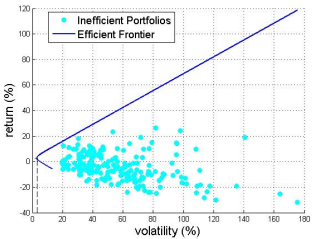
\includegraphics[scale=0.65]{img/Efficient_Frontier.png}
\end{center}
\end{definition}

Note that this efficient portfolio allows us to have unlimited short positions, which may or may not be realistic. If we wanted to work only with all-long portfolios, then we would impose the nonlinear restrictions 
\[0 \leq w_k \leq 1 \text{ for } k = 1, \ldots, K\]
which would need to be solved numerically, possibly using nonlinear models. 

\subsubsection{Efficient Frontier with Risk-Free Asset}

If we include a risk-free asset such as cash $C$ with risk-free return $R_f$ to the portfolio $\{P_1, \ldots, P_K\}$, then we slightly modify our equations. By definition, the risk-free asset has volatility $\sigma_0 = 0$ and its weight must be equal to $w_f = 1 - \sum_{i=1}^K w_k$, so we still want to minimize 
\[\sigma^2 = \frac{1}{2} \mathbf{w}^T \boldsymbol{\Sigma} \mathbf{w}\]
subject to constraint equations 
\[R_f \bigg( 1 - \sum_{k=1}^K w_k \bigg) + \sum_{k=0}^K w_k R_k = R\]
When we allow our portfolio to include the risk-free security, the efficient frontier becomes a straight line that is tangential to the risky efficient frontier and with a $y$-intercept equal to the risk-free rate. 
\begin{center}
    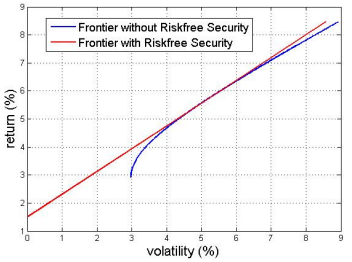
\includegraphics[scale=0.65]{img/Frontier_with_Risk_Free_Sec.png}
\end{center}
We can include other linear portfolio constraints, such as no-borrowing, no-short sales, or certain sector constraints. While analytic solutions are generally no longer available, the resulting problems are easy to solve numerically. 


\subsection{Capital Asset Pricing Model}

Let us have some stock $P$ with random variable of return $R_p = R_{P, [i, j]}$ and the market $M$ with random variable of return $R_m = R_{M, [i, j]}$, both within period $[i, j]$. There may be some sort of risk-free return $r_f$ available (e.g. U.S. treasury bonds), so we can observe the returns of these two assets past the risk-free return by considering the joint distribution 
\[(R_p - r_f) \times (R_m - r_f)\]
This may or may not be correlated, but the capital asset pricing model shows that there exists a linear relationship between the expected values of these two distributions. The central insight of the CAPM is that in equilibrium the riskiness of an asset is not measured by the standard deviation of its return but by its beta. 

\begin{theorem}[CAPM]
Now let $\overline{R}_m = \mathbb{E}[R_m]$ denote the expected return of the market, and $\overline{R} = \mathbb{E}[R]$ denote the expected return of a security or portfolio. Then, the \textbf{capital asset pricing model (CAPM)} asserts that there exists a linear relationship 
\[\overline{R} = r_f + \beta (\overline{R}_m - r_f)\]
where $r_f$ is the risk-free rate. 
\end{theorem}
\begin{proof}
Let us consider a portfolio of weights $\alpha$ and $1 - \alpha$ on the risky security and market portfolio, respectively. Let $R_\alpha$ denote the random return of this portfolio as a function of $\alpha$. We then have 
\begin{align*}
    \mathbb{E}[R_\alpha] & = \alpha \overline{R} + (1 - \alpha) \overline{R}_m \\
    \mathrm{Var}(R_\alpha) & = \alpha^2 \mathrm{Var}(R) + (1 - \alpha)^2 \mathrm{Var}(R_m) + 2 \alpha (1 - \alpha) \mathrm{Cov}(R, R_m)
\end{align*}
Note that as $\alpha$ varies, the mean and standard deviation $(\mathbb{E}[R_\alpha], \mathrm{Var}(R_\alpha))$ trace out a curve in $\mathbb{R}^2$ that cannot cross the efficient frontier, as shown in the dotted line. 
\begin{center}
    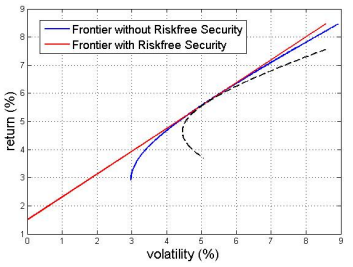
\includegraphics[scale=0.5]{img/CAPM.png}
\end{center}
At $\alpha = 0$, the slope of this curve must equal the slope of the capital market line. The slope of the $\alpha$-curve (where $\sigma(R_\alpha) = \sqrt{\Var(R_\alpha)}$) is 
\begin{align*}
    \frac{d \mathbb{E}[R_{\alpha}]}{d \sigma(R_\alpha)} \bigg|_{\alpha = 0} & = \frac{d\mathbb{E}[R_\alpha]}{d \alpha} \bigg/ \frac{d \sigma(R_\alpha)}{d \alpha} \bigg|_{\alpha = 0} \\
    & = \frac{\sigma(R_\alpha) (\overline{R} - \overline{R}_m)}{\alpha \sigma(R) - (1 - \alpha) \Var (R_m) + (1 - 2 \alpha) \mathrm{Cov}(R, R_m)} \bigg|_{\alpha = 0} \\
    & = \frac{\sigma(R_m) (\overline{R} - \overline{R}_m)}{-\Var(R_m) + \mathrm{Cov}(R, R_m)}
\end{align*}
The slope of the capital market line is $(\overline{R}_m - r_f) / \sigma(R_m)$, and equating the two 
\[\frac{\sigma(R_m) (\overline{R} - \overline{R}_m)}{-\Var(R_m) + \mathrm{Cov}(R, R_m)} = \frac{\overline{R}_m - r_f}{\sigma(R_m)}\]
gives the result. 
\end{proof}



\section{Derivative Markets}

With stocks, we have constructed other securities that are dependent on them, e.g. index funds. These are known as derivatives. 

\begin{definition}[Derivatives]
\textbf{Derivative} investments are investments that are derived, or created, from an underlying asset. Its value $V$ can be derived as a function of the value of the underlying asset $S$ (or a collection of assets $S_1, \ldots, S_n$) and some time variable $t$. For simplicity, we will assume one asset, getting $V(S, t)$. However, since $S_t$ is a stochastic process, our derivative value is also a stochastic process 
\[V_t = V (S_t, t)\]
\end{definition}

Before we talk about derivative valuation and strategies, we must learn to read the following. 

\begin{definition}[Risk Profile Chart] 
The risk profile chart simply just compares the price of our asset (x-axis) and our net profit (y-axis). The horizontal line at $y = 0$ is called the \textbf{breakeven line}. Say the we are longing a stock priced at \$25. Then, our risk profile chart is shown below. Our risk is capped to what we paid, as is our breakeven point, and our potential reward is uncapped. 
\begin{center}
    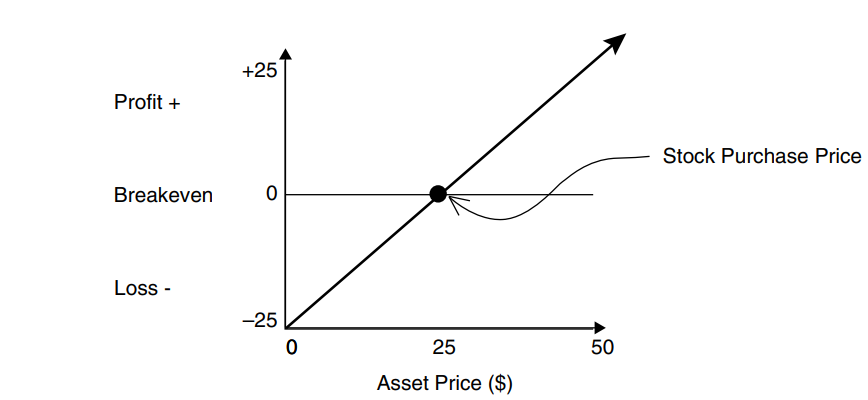
\includegraphics[scale=0.3]{img/risk_long_stock.png}
\end{center}
If we short the same stock, our risk is uncapped as the stock rises, and our potential reward is the price we shorted at, as is our breakeven point. 
\begin{center}
    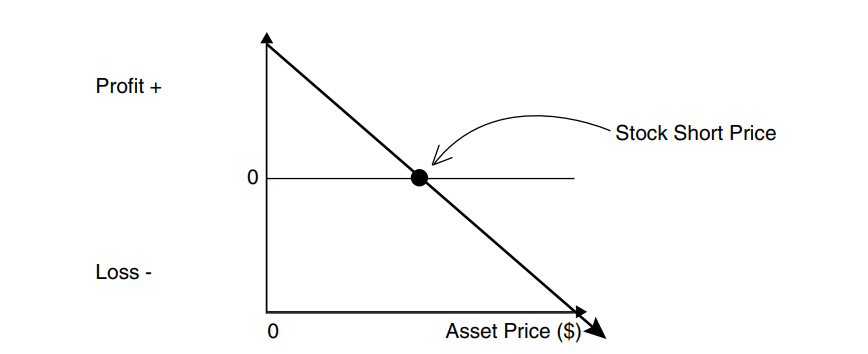
\includegraphics[scale=0.3]{img/risk_short_stock.png}
\end{center}
\end{definition}

What is nice about risk profile charts is that we can graph multiple charts and add them together as if they were functions to look at the risk-profile chart of a portfolio. 

\subsection{Option Contracts}

One type of derivative that we will work with is options. 

\begin{definition}[Put, Call Options]
A \textbf{stock option} is a contract that allows the user to trade an asset 
\begin{enumerate}
    \item at a specific price, called the \textbf{strike price}, and 
    \item within a specific time (for U.S. stocks), called the \textbf{expiration date}. Note that for European ones, they must be exercised at the date, not within. 
    \item a specific number of shares of that asset, called the \textbf{multiplier} (usually, one contract is for 100 shares). 
\end{enumerate}
Buying a \textbf{call option} allows the holder to buy the stock, and a \textbf{put option} allows the holder to sell the stock. 
\end{definition}

A property of options trading is the amount of \textbf{leverage}. One option contract represents 100 shares of stock and is usually a fraction of the cost of what you'd pay for the equivalent number of shares (e.g. 10\% of the actual stock price). Options allow the investor to invest little money with the same potential gains, but options are much more leveraged, i.e. a small investment gives you large market exposures. 

\begin{example}
Say that stock XYZ is trading for \$100. 
\begin{enumerate}
    \item Alice believes that the stock will go up, and so buys a call option to buy 1 share of XYZ at \$120 within 3 months (which costs \$10). If XYZ goes above \$120 (say \$140), then she can execute the contract to buy the stock at \$120 and immediately sell at \$140, making money of \$10. 
    \item Bob believes that the stock will go down, and so buys a put option to sell 1 share of XYZ at \$80 within 3 months (which costs \$10). If XYZ goes below \$80 (say \$60), then he can buy the share at \$60 and execute the contract to sell it at \$80, making money of \$10. 
\end{enumerate}
Note that neither Alice nor Bob had to invest too much money to bet on their strategies. They only had to spend \$10, rather than the \$100 for the stock. 
\end{example}

\begin{definition}[Time Decay]
So far, we have ignored the effects of the expiration date, which can be modeled with a \textbf{time decay} model. That is, we must consider the probabilities of the underlying asset's price moving in or against our favor during the time remaining. The more time remaining, the more potential volatility. In general, 
\begin{enumerate}
    \item time decay \textit{hurts} us when we buy options since as time passes, we have less time to be right. So we don't like to own options during the last month. 
    \item time decay \textit{helps} us when we sell options. 
\end{enumerate}
\end{definition}

In general, options with a shorter expiration date are less valuable since they give the investor little time to be correct. But don't be fooled by the false economy that shorter options are cheaper. Comparing a 1-month to a 12-month option and dividing the long option price by 12 gives you far less per month. 

\subsubsection{Four Basic Options Trading}

For longing options, we buy options and hold them in hopes that the stock direction will move in our favor. With long options, we can limit our downside to whatever we paid for the option. 

\begin{definition}[Long Call Option]
We buy a call option with strike price of \$100 at \$10. As of now, our option is worthless and we have a net profit of -\$10. However, if the underlying asset increases in value past \$110, then we have a net profit since we can exercise the option right away to make money. Note that our profits are unlimited since the price of the underlying asset is unlimited, and our losses are capped at \$10. 
\begin{center}
    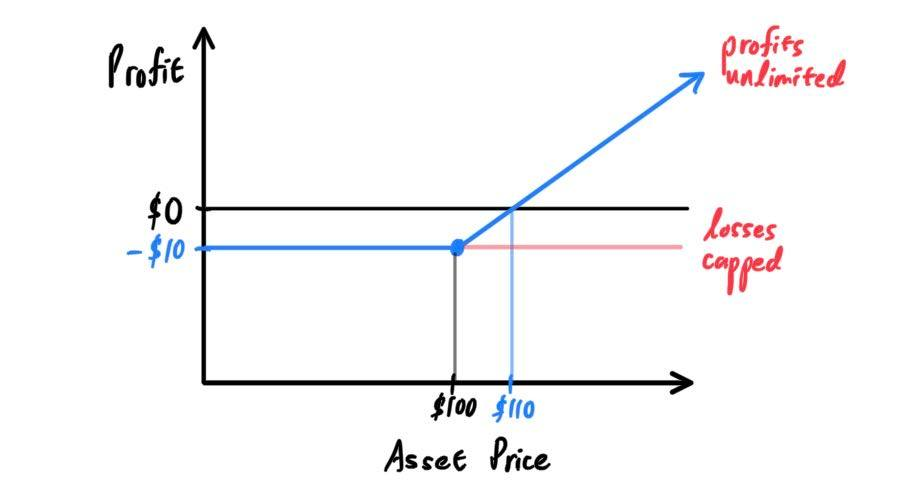
\includegraphics[scale=0.3]{img/long_call.jpg}
\end{center}
Let the current stock price be $S$ and the strike price of the option be $X$, then the intrinsic value of this call is 
\[\max\{S - X, 0\}\]
\end{definition}

\begin{definition}[Long Put Option]
Long put option: We buy a put option with strike price of \$100 at \$10. As of now, our option is worthless and we have a net profit of -\$10. However, if the underlying asset decreases in value past \$90, then we have a net profit since we can exercise the option right away to make money. Note that our profits are maxed at \$90 since the price of the underlying asset can fall past \$90 to \$0, and our losses are capped at \$10. 
\begin{center}
    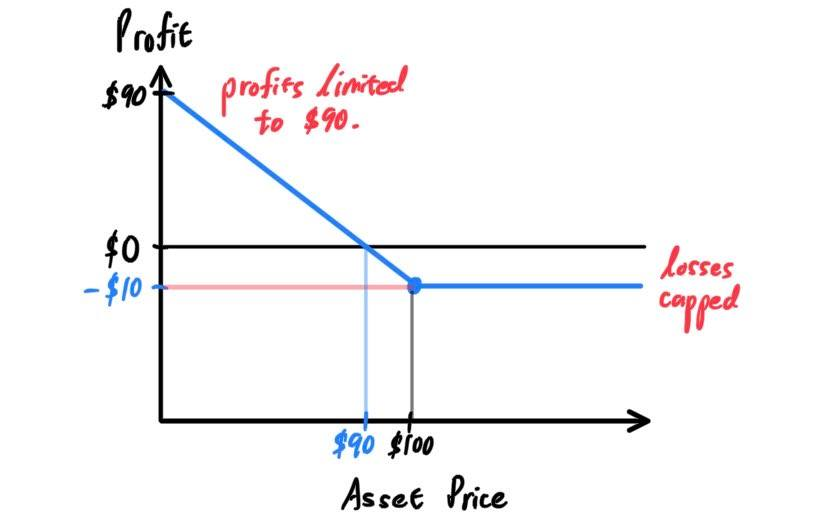
\includegraphics[scale=0.3]{img/long_put.jpg}
\end{center}
Let the current stock price be $S$ and the strike price of the option be $X$, then the intrinsic value of this put is 
\[\max\{X - S, 0\}\]
\end{definition}

\begin{definition}[In/Out/At of Money]
Given an option, 
\begin{enumerate}
    \item if its intrinsic value is positive, then we say it is \textbf{in the money (ITM)}. 
    \item if its intrinsic value is negative, then we say it is \textbf{out of money (OTM)}. 
    \item if the strike price $X$ is the identical to the current price $S$ of the underlying asset, then we say it is \textbf{at the money (ATM)}. 
\end{enumerate}
\end{definition}

For shorting options, just like shorting stocks, we borrow options and sell them immediately for \$10 in hopes that their value will go down. The value can go down in two ways: when we sell a call option and the stock price goes down, or when we sell a put option and the stock price goes up. We can then buy it back at the decreased market price and return to the borrower. 

\begin{definition}[Short Call Option]
Short call option: We borrow a call option with strike price of \$100 and immediately sell it at \$10. We hope that the underlying asset will stay at or below \$100, rendering the value of the call to be \$0. If it stays at \$0, then we can buy it back and return \$0 to the borrower, making \$10. If the underlying asset goes to \$105, then the option value is \$5, and we can get a \$5 profit. However, the underlying asset can increase in value arbitrarily, meaning that our losses are unlimited. 
\begin{center}
    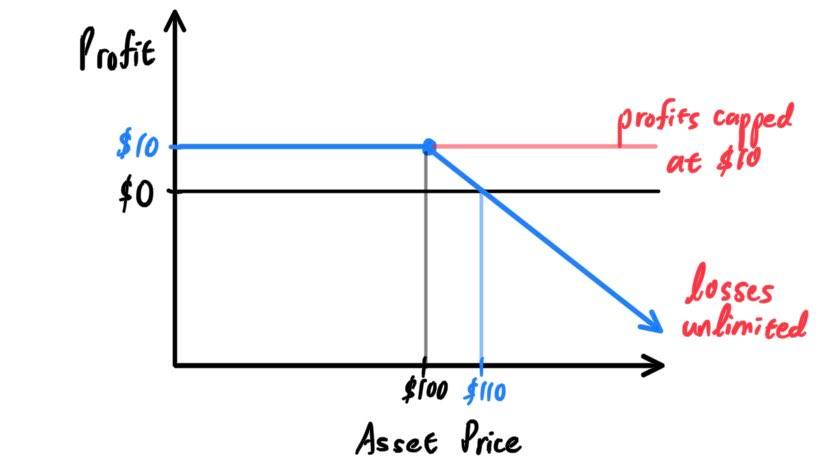
\includegraphics[scale=0.3]{img/short_call.jpg}
\end{center}
\end{definition}

\begin{definition}[Short Put Option]
Short put option: We borrow a put option with strike price of \$100 and immediately sell it at \$10. We hope that the underlying asset will stay at or above \$100, rendering the value of the put to be \$0. If it stays at \$0, then we can buy it back and return \$0 to the borrower, making \$10. If the underlying asset goes to \$95, then the option value is \$5, and we can get a \$5 profit. Note that the underlying asset can decrease in value to \$0, so our losses are maxed at \$90. 
\begin{center}
    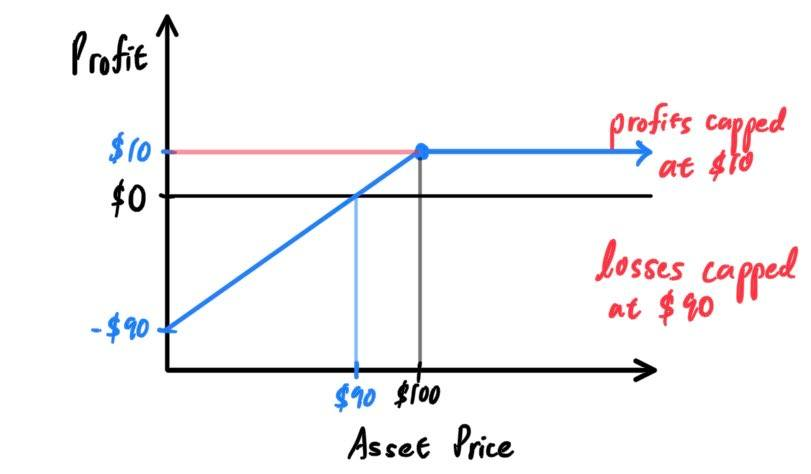
\includegraphics[scale=0.3]{img/short_put.jpg}
\end{center}
\end{definition}

\subsection{Black Scholes Model}

Now, we can talk about how to price European options. Note that due to the fact that we can exercise American options before their expiration date, more complex models are required for them, but it is often the case that funds use Black-Scholes to value them too. 

\begin{definition}[Martingale and Arbitrage Free Pricing]
Assume that the stock $S_t$ is a stochastic process following a geometric Brownian motion 
\[\frac{d S_t}{d t} = r \, dt + \sigma \, dW(t)\]
consisting of a drift term $r \,dt$ and Brownian motion $dW(t)$ of variance $\sigma^2 dt$ over a small period of time $dt$. Then, the value of a call option and a put option are the stochastic processes: 
\begin{align*}
    C_t & = e^{-r (T - t)} \, \mathbb{E}[\max\{S_T - X, 0\}] \\
    P_t & = e^{-r (T - t)} \, \mathbb{E}[\max\{X - S_T, 0\}]
\end{align*}
where $X$ is the strike price and $T$ is the maturity. Note that $S_T$ is the only random variable here.
\end{definition}

\begin{definition}[Black-Scholes Formula]
Given that we have 
\begin{enumerate}
    \item the underlying asset's price $S_t$ (which is a random variable) and its volatility $\sigma$ (which can be estimated by taking the standard deviation of historical log returns)
    \item the option, with strike price $X$ and maturity in years $T$ 
    \item the risk free rate $r$ 
\end{enumerate}
we can price this option using the \textbf{Black-Scholes Options Pricing Formula} as 
\[C_t = \Phi (d_1) \, S_t - \Phi(d_2) \, X \, e^{-r (T - t)}\,\]
where 
\[d_1 = \frac{ \ln \big(\frac{S_t}{X} \big) + \big( r + \frac{\sigma^2}{2} \big) (T - t)}{\sigma \sqrt{T - t}} \text{ and } d_2 = d_1 - \sigma \sqrt{T - t}\]
and $\Phi$ is the CDF of the standard normal distribution. Note that this Black-Scholes equation is really just a time-paramaterized function of 
\[C_t ( S_t, \sigma, X, T, r)\]
with the properties: 
\begin{enumerate}
    \item This is a monotonically increasing function of $\sigma$. We can see this because the greater the price movements of a stock, the more changes those large moves will produce an in-the-money option. 
\end{enumerate}
\end{definition}

This allows us to price options simply by plugging in the necessary values above, and this should equal the market price $P$ of the option. Often, this is not the case. 
\[C_t ( S_t, \sigma, X, T, r) \neq P\]
If we assume that the Black-Scholes model perfectly values options prices, it has to be due to an inaccuracy in our parameters. The only parameter not readily available as an input into the equation is volatility, so we can modify that. 

\begin{definition}[Implied Volatility]
The \textbf{implied volatility} of an option contract is the theoretical volatility $\sigma$ of the underlying instrument s.t. the Black-Scholes pricing model equals the current market price of the option. That is, taken $S_t, X, T, r$ to be constant, it is the value of $\sigma$ s.t. 
\[C_t (S_t, \sigma, X, T, r) = P \]
In essence, the implied volatility acts as the expected volatility of the stock during the time period from now $t$ until expiration $T$. The greater this implied volatility is, the more changes that the option will be ITM, and the higher value it will have. 
\end{definition}

\begin{enumerate}
    \item If the implied volatility is greater than the historical volatility, we expect there to be greater volatility in the underlying asset compared to the historical volatility, and so we should see that 
    \[C_t (S_t, \sigma, X, T, r) < P \]
    \item If it is less, then we expect there to be less volatility in the underlying asset, and so 
    \[C_t (S_t, \sigma, X, T, r) > P \]
\end{enumerate}
Surprisingly, it turns out that most of the time, the implied volatility is greater than the historical volatility, an phenomenon we will explain now. 

\begin{definition}[Volatility Risk Premium]
The \textbf{volatility risk premium (VRP)} refers to the following two phenomenon, which are equivalent due to monotonicity of $C_t$ w.r.t. $\sigma$: 
\begin{enumerate}
    \item Option-implied volatility tends to exceed realized volatility of the same underlying asset over time.  
    \item The market price $P$ of the option tends to exceed the Black-scholes pricing $C(S_t, \hat{\sigma}, X, T, r)$, where $\hat{\sigma}$ is the historical volatility. 
\end{enumerate}
To explain this, a study from Yale suggests that market participants tend to overestimate the probability of a significant crash, leading to higher demand for options. This heightened perception of risk may lead to higher willingness to pay for these options to hedge a portfolio, which is realized in the additional premium $P - C(S_t, \hat{\sigma}, X, T, r)$. 
\end{definition} 

\subsubsection{Volatility Smile and Skew}

Let us have two options for the same underlying asset $S_t$ and the same strike price $T$, with two different strike prices $X_1$ and $X_2$, and option market price $P_1, P_2$. Then, the Black-Scholes model assumes that the implied volatility $\sigma_1$ and $\sigma_2$ are equal, and that it is only the difference in strike prices that causes $P_1 \neq P_2$. 
\[\sigma_1 = \sigma_2\]
This makes sense, since no matter what option we are looking at, the underlying asset is the same and so should our estimate of its implied volatility be. Therefore, our strike price vs implied volatility chart should look like a straight line (given that underlying asset and strike price are the same). 
\begin{center}
%    \includegraphics[scale=0.3]{}
\end{center}

However, empirically, this is not the case. 

\begin{definition}[Volatility Smile]
A situation in which at-the-money options have lower implied volatility than out-of-the-money or in-the-money options is sometimes referred to as a volatility "smile" due to the shape the data creates when plotting implied volatilities against strike prices on a chart. In other words, a volatility smile occurs when the implied volatility for both puts and calls increases as the strike price moves away from the current stock price, i.e. they predict a higher expected volatility of the underlying asset in the remaining period $[t, T]$. This means that as the strike price moves away from the current stock price, the price of the options are in fact higher than what is accounted for in the Black-Scholes model. 
\begin{center}
%    \includegraphics[scale=0.3]{}
\end{center}
\end{definition}

Why is this true? Volatility smiles started occurring in options pricing after the 1987 stock market crash. They were not present in U.S. markets beforehand, indicating a market structure more in line with what the Black-Scholes model predicts. After 1987, traders realized that extreme events could happen and that markets have a significant skew (fat-tailed towards these extreme events). The possibility for extreme events needed to be factored into options pricing. Therefore, in the real world, implied volatility increases or decreases as options move more ITM or OTM. 

\begin{example}[EDIT]
Say that stock XYZ is priced at \$100. Say that a massive movement happens of the stock jumping \$40, with a downside of probability 50\% and upside with probability of 50\%. 
\begin{enumerate}
    \item You have a call option with strike price \$120, which is OTM and has \$0 intrinsic value. If a massive market movement happens, then a downside won't affect you will render your intrinsic option value to be \$0, and an upside will cause it to be \$20 with 0.5 probability. Therefore, you expect to make \$10 gains.  
    \item You have a call option with strike price \$80, which is ITM and has \$20 intrinsic value. If a massive market movement happens, then a downside will cause your intrinsic option value to be \$0 and an upside will cause it to be \$60. Therefore, you expect the value to be \$30, and therefore make \$10 gains. 
    \item You have a call option with strike price \$100, which it ATM and has \$0 intrinsic value. If a massive market movement happens, then a downside won't affect you a
\end{enumerate}
\end{example}

The volatility smile is not predicted by the Black-Scholes model, which is one of the main formulas used to price options and other derivatives. The Black-Scholes model predicts that the implied volatility curve is flat when plotted against varying strike prices. Based on the model, it would be expected that the implied volatility would be the same for all options expiring on the same date with the same underlying asset, regardless of the strike price. 

\begin{definition}[Volatility Skew]
A \textbf{volatility skew} describes the observation that not all options on the same underlying and expiration have the same implied volatility assigned to them in the market. Rather, the curve is "skewed" to the right because investors are willing to pay for a lower strike option to protect them against a market downturn. 
\begin{center}
%    \includegraphics[scale=0.3]{}
\end{center}
\end{definition}



\subsection{Greeks}

\begin{definition}[Delta]
The \textbf{Delta} of a financial derivative is the rate of change of the value with respect to the value of the underlying security.
\[\Delta_t = \frac{\partial V_t}{\partial S_t}\]
It indicates how many options contracts are needed to hedge a long or short position in the underlying asset. 
\begin{enumerate}
    \item For a call option, the delta would be in $[0, 1]$
    \item For a put option, the delta would be in $[-1, 0]$
\end{enumerate}
If means that for every \$1 increase in stock price, the option price increases roughly by $\$\Delta$, with all else being equal.  
\end{definition}

\begin{definition}[Gamma]
The \textbf{Gamma} of a derivative is the sensitivity of $\Delta$ with respect to $S$. 
\[\Gamma_t = \frac{\partial^2 V_t}{\partial S_t^2}\]
It measure the rate of change of Delta. 
\end{definition}

The following diagram represents how delta and gamma changes as time moves forward. 
\begin{center}
    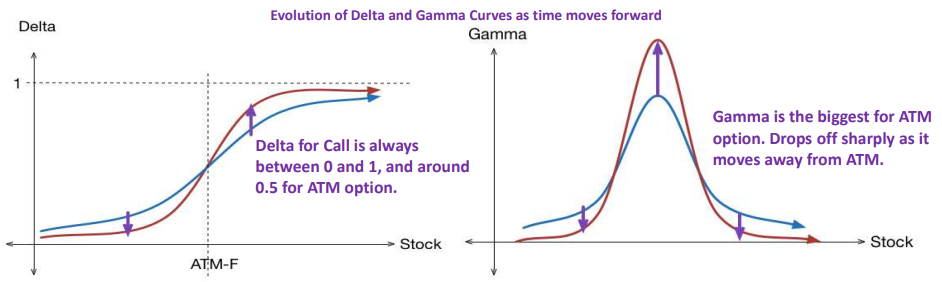
\includegraphics[scale=0.4]{img/delta_gamma_as_time_increases.png}
\end{center}

\begin{definition}[Theta]
The \textbf{Theta} of is 
\[\Theta_t = \frac{\partial V_t}{\partial t}\]
It measures the impact of a change in time remaining. 
\end{definition}

\begin{definition}[rho]
The \textit{rho} of a derivative security is the rate of change of its value with respect to the interest rate $r$
\[\rho_t = \frac{\partial V_t}{\partial r}\]
\end{definition}

\begin{definition}[Vega]
The \textbf{Vega} of a derivative is the rate of change of the derivative with respect to the volatility $\sigma$ of the underlying asset 
\[\Lambda_t = \frac{\partial V_t}{\partial \sigma}\]
\end{definition}

\begin{theorem}
Given the Black-Scholes model, we can derive the following formulas: 
\begin{align*}
    \text{Call } \Delta_t & = \frac{\partial C_t}{\partial S_t} = \Phi(d_1) \\
    \text{Put } \Delta_t & = \frac{\partial P_t}{\partial S_t} = 1 - \Phi(d_1) \\
    \Gamma_t & = \frac{\partial^2 C_t}{\partial S_t^2} = \frac{\partial^2 P_t}{\partial S_t^2} = \frac{1}{S_0 \sigma \sqrt{T - t}} \frac{1}{\sqrt{2\pi}} e^{- d_1^2 / 2} \\
    \Lambda_t & = \frac{\partial C_t}{\partial \sigma} = \frac{\partial P_t}{\partial \sigma} = S_0 \sigma \sqrt{T - t} \frac{1}{\sqrt{2\pi}} e^{-d_1^2 / 2} = \sigma^2 (T - t) \Gamma_t 
\end{align*}
\end{theorem}

\subsection{Forward/Future Contracts}

Another type of derivative that we will work with is forwards and futures. 

\begin{definition}[Forward Contract]
A \textbf{forward contract} is an obligation to trade a certain asset 
\begin{enumerate}
    \item at a specific price, called the \textbf{forward price}, and 
    \item at a specific time, called the \textbf{expiration date} 
    \item a specific number of assets, called the \textbf{multiplier}
\end{enumerate}
They are typically not traded on exchanges, but rather \textbf{over the counter (OTC)} between two private parties. 
\end{definition}

Note that both sellers and buyers forward contracts are involved in a forward transaction and are both \textit{obligated} to fulfill their end of the contract at maturity. This induces a significant counterparty risk of failure to deliver and low trading volume/liquidity. 

\begin{definition}[Future Contracts]
A \textbf{future contract} is the same as forward contracts (with the execution price called the \textbf{future price}), except that 
\begin{enumerate}
    \item futures are settled daily (not just at maturity), meaning that futures can be bought or sold at any time 
    \item Futures are standardized and typically traded on public exchanges, with greater price transparency and liquidity
\end{enumerate}
\end{definition}

\noindent There are broad asset classes for future markets, which include 
\begin{enumerate}
    \item agricultural commodities e.g. corn, wheat, livestock 
    \item energy products, e.g. crude oil, gasoline, heating oil
    \item metals, e.g. gold, silver, copper 
    \item financial products 
    \begin{enumerate}
        \item equities - S\&P index, single stocks 
        \item interest rates - treasury bonds, swaps 
        \item foreign exchanges 
        \item volatility 
    \end{enumerate}
    \item options on futures, which give you the right but not the obligation to enter into a future contract at an agreed price 
\end{enumerate}
When you buy a futures contract and it matures, it can either be settled physically by delivering the underlying commodity like oil, sugar, wheat, etc. or it can be settled in cash by paying/receiving the price differences between the final trading price and your initial transaction price. Since most retail traders do not have the resources to allocate these commodities, the vast majority of futures contracts never takes physical delivery, and they are automatically sold right before it matures to avoid taking delivery of the oil. 

\subsubsection{Valuation of Forward/Futures Contracts}

The forward/future prices are determine in real trading by supply and demand similar to options and stocks. The difference between forward and futures price is primarily driven by future interest rates. Given the short tenor of forward contracts, the difference is not big, but could be material on a large notional contract. 

The theoretical forward/future prices can be calculated as such. Let $X$ be the fair forward/future price agreeable to both parties. Then, the price of the contract at time $t$ should be the current value $S_t$ (which we assume to follow geometric Brownian motion) of the underlying asset minus an exponentially decaying $X$. 
\[S_t - e^{-r (T - t)} X\]

\subsubsection{Cost-of-Carry Model and Futures Arbitrage}

Suppose that you want to sell a commodity A forward in 3 months. One way to fulfill our obligation is to buy A today, store it for 3 months, and sell it at the end of the period. The contracts to buy and sell today (generally with a few days of delivery period) are called \textbf{spot contracts}. 

\begin{definition}[Cost-of-Carry Pricing Model]
As such, a futures price should simply be the spot price plus the cost of carrying inventory forward. This is generally called the \textbf{cost-of-carry pricing model} for futures. 
\[\text{Futures Price} = \text{Spot Price} + \text{Carry Cost}\]
The carry cost normally includes cost of storage, insurance, potential damage (e.g. perishable goods). The future price can be higher or lower than the spot price. 
\begin{enumerate}
    \item If the future price is lower than the spot price, we have a \textbf{backwardation market}. 
    \item If the future price is higher than the spot price, we have a \textbf{contango market}. 
\end{enumerate}
This gives us an arbitrage opportunity as we can long one and short the other, given that we can accurate determine the carry cost. 
\end{definition}


\section{Derivative Trading Strategies}

\subsection{Covered and Protective Calls and Puts}

\begin{definition}[Covered Call]
If you long stock XYZ, you can achieve a \textbf{covered call} by shorting a call option on the stock that you already own, i.e. selling someone else the right to buy a stock you own. The investor's long position in the asset is the \textit{cover} because it means the seller can deliver the shares is the buyer of the call option chooses to exercise. 

By shorting the call, we limit our upside (since $S_t$'s price rising will cancel out with the value of the short call), but we can reap the premium for selling the option. In this end, this is a long position, since we are betting that the stock will stay high enough so that we can consistently collect the premium. 
\begin{center}
    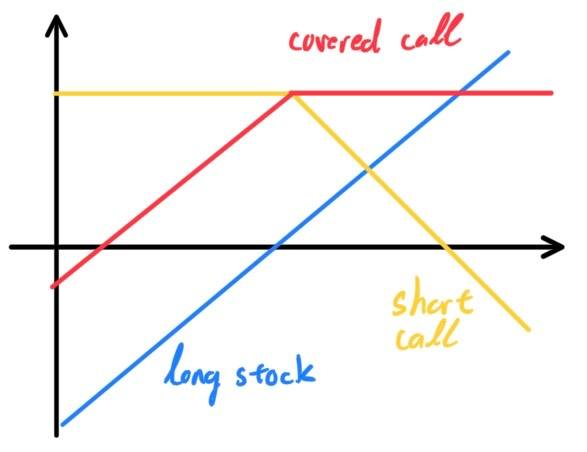
\includegraphics[scale=0.3]{img/covered_call.jpg}
\end{center}
A covered call is similar to a short put. 
\end{definition}

\begin{definition}[Covered Put]
If you short stock XYZ, you can achieve a \textbf{covered put} by shorting a put option on XYZ. By shorting the put, we limit our upside, but as long as the stock stays low enough, we can collect our premium for selling the option. 
\begin{center}
    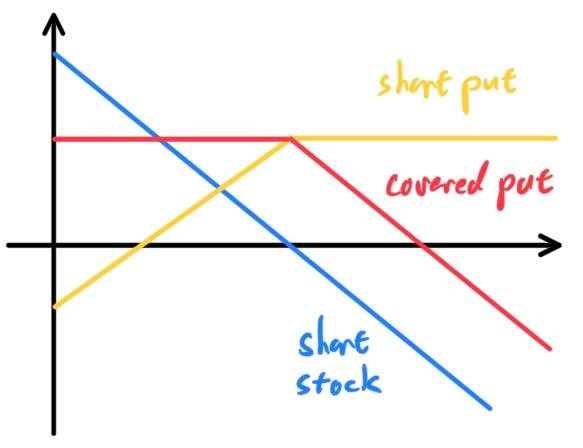
\includegraphics[scale=0.3]{img/covered_put.jpg}
\end{center}
A covered put is similar to a short call. 
\end{definition}

\begin{definition}[Protective Put]
If you long stock XYZ, you can achieve a \textbf{protective put} by longing a put option. By longing the put, we protect our downside, but lose a bit of our upside potential. 
\begin{center}
    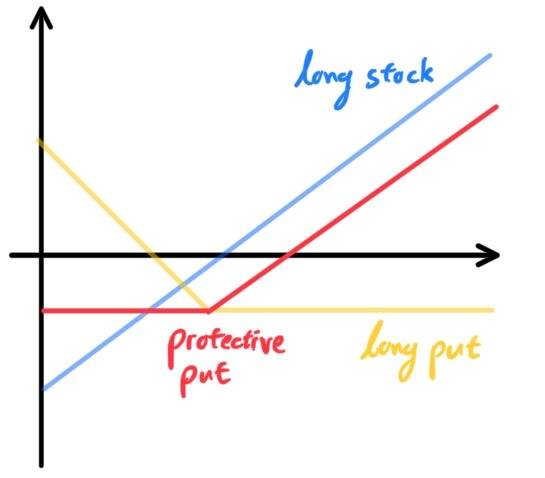
\includegraphics[scale=0.3]{img/protective_put.jpg}
\end{center}
It is similar to a long call option. 
\end{definition}

\begin{definition}[Protective Call]
If you short stock XYZ, you can achieve a \textbf{protective call} by longing a call option. By longing the put, we protect our downside, but lose a bit of our upside potential. 
\begin{center}
    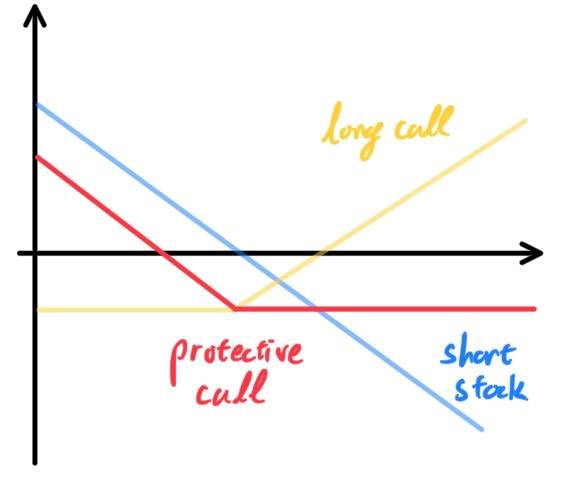
\includegraphics[scale=0.3]{img/protective_call.jpg}
\end{center}
It is similar to a long put option. 
\end{definition}

\subsection{Delta Hedging}

\begin{definition}[Delta Hedging]
\textbf{Delta hedging} is the process of dynamically hedging the option position with the underlying stocks. Given the nonlinearity, the hedge ratio has to be adjusted dynamically. For example, to hedge a short call option, we need to buy $\Delta$ amount for stock for each option. The resulting portfolio 
\[V_t = -C_t + \Delta S_t\] 
has the first derivative $0$, which is called \textbf{delta neutral}. However, as $S_t$ changes, the $\Delta_t$ changes by the amount of $\Gamma_T \Delta_t S_t$. That means 
\begin{enumerate}
    \item when the price goes up, we need to buy more shares, and 
    \item when the prices goes down, we need to sell more shares. 
\end{enumerate}
\end{definition}

If we perform delta hedging strategy continuously, we would have 
\[\text{PnL} = \int_0^T \frac{S_t^2}{2} \Gamma_t (\sigma_{\text{implied}}^2 - \sigma_{\text{realized}}^2 )\, dt\]

\subsection{Volatility Trading Strategies}
We will talk about three volatility trading strategies. 
\begin{enumerate}
    \item Long straddles 
    \item long strangles 
    \item long butterfly spreads
\end{enumerate}

\begin{definition}[Long Straddle]
A \textbf{long straddle} is achieved when you buy a call option and a put option at the same strike price $X$ and expiration date. Assume you paid $P$ for each of these options. Then, 
\begin{enumerate}
    \item if the underlying asset $S_t \in [X - 2P, X + 2P]$, then for one of the options, we make $|S_t - X|$ and $0$ for the option, minus $2P$ for initially buying. This results in a loss: 
    \[|S_t - X| - 2P \leq 2P - 2P = 0 \]
    \item if $S_t > X + 2P$, then you make $S_t - X$ money on the call, and $0$ on the put, so a total profit of 
    \[S_t - X - 2P > 2P - 2P > 0\]
    
    \item if $S_t < X - 2P$, then you make $X - S_t$ money on the put, and $0$ on the call, so a total profit of 
    \[X - S_t - 2P > 2P - 2P > 0\]
\end{enumerate}
Either way, as long as $S_t$'s change is dramatic (i.e. volatile) past $\pm 2P$ in either direction, we can see that this will generate profits. 
\begin{center}
    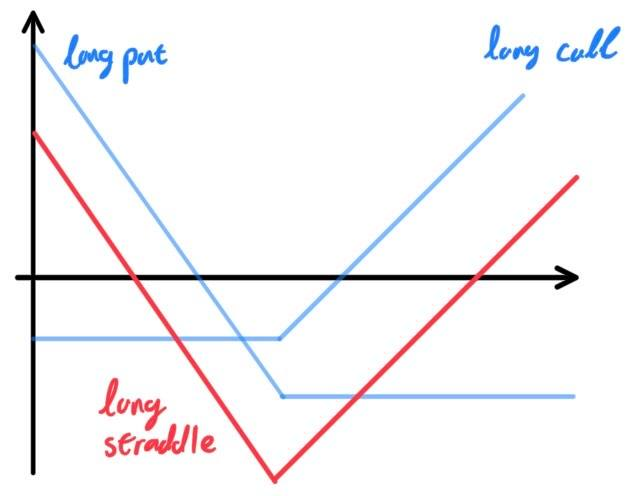
\includegraphics[scale=0.3]{img/long_straddle.jpg}
\end{center}
\end{definition}

\begin{definition}[Long Strangle]
A \textbf{long strangle} is achieved when you buy a call and a put option at \textit{different} strike prices $X_c$ and $X_p$ (usually both out-of-money) and the same expiration date. Assume you paid $P$ for each of these options. Assume they are both out-of-money, meaning that $X_p < S_t < X_c$
\begin{enumerate}
    \item if $S_t \in [X_p - 2P, X_c + 2P]$, then for one of the options, we make at most $2P$ and $0$ for the other, resulting in a loss. 
    \item If $S_t > X_c + 2P$, then you make $S_t - X_c$ money on the call, and $0$ on the put, so a total profit of 
    \[S_t - X_c - 2P > 2P - 2P > 0\]
    
    \item If $S_t < X_p - 2P$, then you make $X_p - S_t$ money on the put, and $0$ on the call, so a total profit of 
    \[X_p - S_t - 2P > 2P - 2P > 0\]
\end{enumerate}
Either way, as long as $S_t$'s change is dramatic (i.e. volatile) past $\pm 2P$ in either direction past the respective strike prices, we can see that this will generate profits. 
\begin{center}
    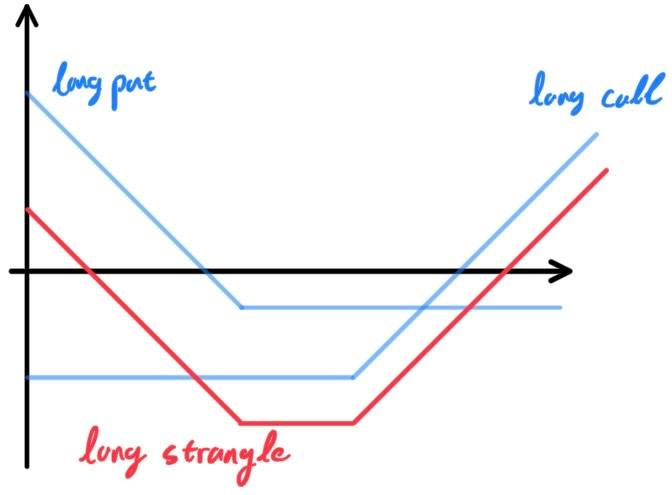
\includegraphics[scale=0.3]{img/long_strangle.jpg}
\end{center}
\end{definition}

A long strangle may be preferred to the long straddle because since both are OTM, we pay a smaller premium for them (and you are going to have less money exposed to time decay). Furthermore, even though you are not maximizing your exposure to volatility, you have smaller loss potential. The following fact quantifies the differences between the straddle and the strangle. 

\begin{theorem}
The straddle will always have a higher gamma than the strangle and therefore will be more appropriate for traders who are betting on an increase in the actual volatility of the market. 
\end{theorem}

It is important that the trader remains disciplined. You must place the trades as a spread and take them off as a spread. If one starts looking at each component separately and trades them not as a spread but one at a time, things can get very dangerous. What may occur is that the underlying market jolts one way or the other, and you will be very tempted to take off only one side of the spread. For example, consider that we bought a straddle and the market collapsed, we might want to take off the call and let the put "ride". What usually happens is that then the market will rally and you lose on both the call and the put. 

\begin{definition}[Short Straddle]
Short selling a straddle implies that you are betting against the fact that the market will be volatile. You want to borrow both call and put options with strike price $X$ and sell each of them at $P$. So now, we have $2P$ in cash. 
\begin{enumerate}
    \item if $S_t \in [X - 2P, X + 2P]$, then one of the options is worth at most $2P$ and the other is worthless. We buy them back at the discounted price and give them back to the lender, generating profits. 
    
    \item If $S_t \not\in [X - 2P, X + 2P]$, then one of the options is worth more than $2P$ and the other is worthless, meaning that it takes more cash to buy them back than what we sold them for, resulting in a loss. 
\end{enumerate}
Its risk profile chart indicates that the risk is unlimited. 
\begin{center}
    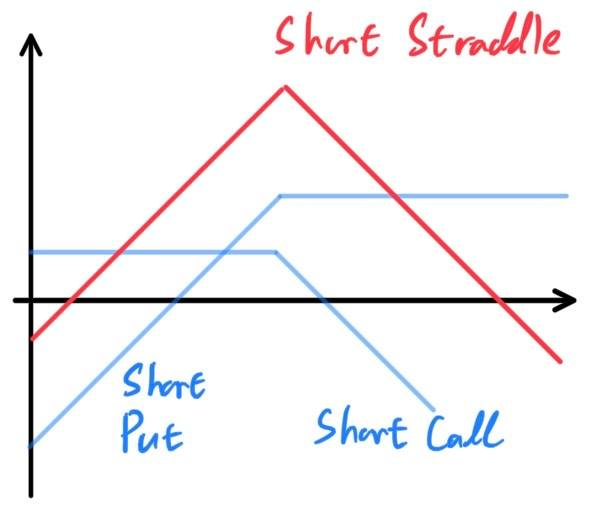
\includegraphics[scale=0.3]{img/short_straddle.jpg}
\end{center}
\end{definition}

\begin{definition}[Short Strangle]
Short selling a strangle is similar. You want to borrow both call and put options with strike price $X_c$ and $X_p$ (assuming $X_p < S_t < X_c$) and sell each of them at $P$. So now, we have $2P$ in cash. 
\begin{enumerate}
    \item if $S_t \in [X_p - 2P, X_c + 2P]$, then one of the options is worth at most $2P$ and the other is worthless. We buy them back at the discounted price and give them back to the lender, generating profits. 
    
    \item If $S_t \not\in [X_p - 2P, X_c + 2P]$, then one of the options is worth more than $2P$ and the other is worthless, meaning that it takes more cash to buy them back than what we sold them for, resulting in a loss. 
\end{enumerate}
Its risk profile chart indicates that the risk is unlimited. 
\begin{center}
    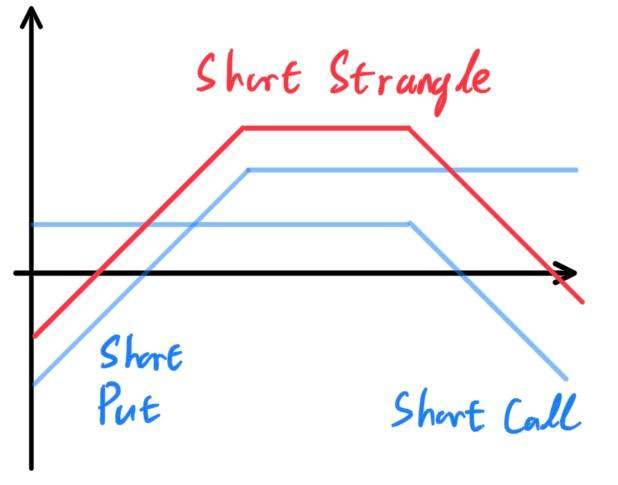
\includegraphics[scale=0.3]{img/short_strangle.jpg}
\end{center}
\end{definition}

Conservative traders who do not like the unlimited risk associated with shorting options can use a butterfly spread to limit their loss potentials. It is a short volatility strategy that makes money from volatility decreasing but mostly from time decay. We can construct butterfly spreads with long calls, long puts, short calls, and short puts, but we will only introduce long calls here. 

\begin{definition}[Long Call Butterfly Spread]
With a butterfly, 
\begin{enumerate}
    \item long a call option with a relatively low strike price $X_1$ 
    \item long a call option with a relatively high strike price $X_3$ 
    \item short two call options (near ATM) with strike price $X_2$, halfway in between $X_1$ and $X_3$. 
\end{enumerate}
Let the current price of the underlying asset be $S_t$ and $P$ be the price for each of the options. 
\begin{enumerate}
    \item If $S_t < X_1$, then you make no money on either long (and we paid $2P$ for them), and for the short calls we get a profit of $2P$. This results in a net $0$ profit. 
    \item If $X_1 < S_t < X_2$, then you make $S_t - X_1$ on the first long, $0$ on the second long, and $2P$ for the shorts. So a profit of 
    \[(S_t - X_1) + 2P - 2P = S_t - X_1 \]
    \item If $X_2 < S_t < X_3$, then you make $S_t - X_1$ on the first long, $0$ on the second long, and lose $2 (S_t - X_2)$ for the shorts. So a total profit of 
    \[(S_t - X_1) - 2 (S_t - X_2) - 2P = - S_t - X_1 + 2X_2 - 2P\]
    \item If $X_3 < S_t$, then you make $S_t - X_1$ on the first long, $S_t - X_3$ on the second long, and lose $2 (S_t - X_2)$ for the shorts. So a total profit of  
    \[(S_t - X_1) + (S_t - X_3) - 2 (S_t - X_2) - 2P = -2P\]
\end{enumerate}
Clearly, our assumptions on the prices $P$ being equal are too strong, which results in the asymmetricity of the risk-profile chart. In reality, the risk profile chart will be symmetric. 
\begin{center}
    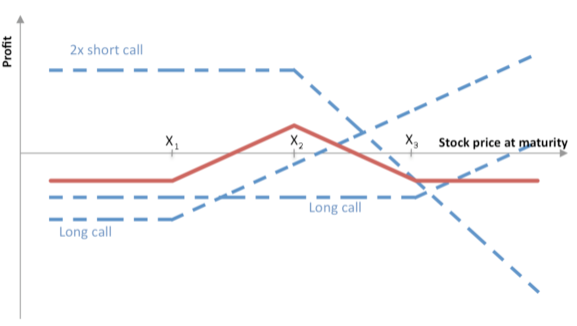
\includegraphics[scale=0.5]{img/butterfly_long.png}
\end{center}
\end{definition}

They are also brilliant from a time decay standpoint, especially in the last 30 days. They decay at an extraordinary rapid pace in the last 30 days. So these trades are ideal to reap the rewards of heavy time decay without having to assume an unreasonable amount of risk. 

\subsection{Dispersion Trading}

Take $X_1, \ldots, X_n$ iid and bounded on compact $D \subset \mathbb{R}^d$. Define $f: D^n \rightarrow \mathbb{R}$
\[f(x_1, \ldots, x_n) = \frac{1}{_n C_2} \sum_{i, j} ||x_i - x_j||_p\]
for $1 \leq p \leq \infty$ be the average distance between two vectors. $f$ is $L$-Lipschitz, and so 
\[\mathbb{P} \big( |f(X_1, \ldots, X_n) - \mu| \geq t \big) \leq \exp \bigg( - \frac{2t^2}{L^2 C} \bigg), \;\;\;\;\; C = \mathrm{diam}(D)\]


\end{document}
